\documentclass[fontsize=12pt,paper=a4,twoside]{scrartcl}

\usepackage{longtable}

\usepackage{graphicx}
\usepackage{rotating}
\usepackage{pdflscape}
\usepackage[normalem]{ulem}
\useunder{\uline}{\ul}{}

% SWP-Präambel
% C 2003-2017 Sebastian Offermann, Rainer Koschke, Karsten Hölscher
% In Zeilen 40 und 41 sind jeweils die aktuellen Daten einzutragen

\usepackage[utf8]{inputenc}     % Kodierung der Tex-Datei
\usepackage[T1]{fontenc}        % Korrekte Ausgabe von Sonderzeichen (Umlaute)
\usepackage[ngerman]{babel}     % Deutsche Einstellungen [ab \begin{document}]

\usepackage{bibgerm}            % Bibliographie
\usepackage{fancyhdr}           % obere Seitenränder gestalten
\usepackage{float}              % Floats Objekte mit [H] festsetzen
\usepackage{graphicx}           % Graphiken als jpg, png etc. einbinden
\usepackage{moreverb}           % zusätzliche verbatim-Umgebungen
\usepackage{pdflscape}          % PDF-Support für landscape
\usepackage[final]{pdfpages}    % Externe PDFs einbinden
\usepackage{stmaryrd}           % zusätzliche Symbole
\usepackage{supertabular}       % Tabellen über Seitenränder hinaus
\usepackage{tabularx}           % Tabellen mit vorgegebener Breite
\usepackage{url}                % setzt URLs schön mit \url{http://bla.laber.com/~mypage}

%%% Die Reihenfolge der folgenden Pakete muss beibehalten werden:
%%% varioref, hyperref, cleveref, bookmark
% Verweise innerhalb des Dokuments schick mit " ... auf Seite ... "
% automatisch versehen. Dazu \vref{labelname} benutzen
\usepackage[ngerman]{varioref}  % [vor hyperref für korrekte Verweise]
\usepackage[colorlinks=true, pdfstartview=FitV, linkcolor=blue,
            citecolor=blue, urlcolor=blue, hyperfigures=true,
            pdftex=true]{hyperref} % [vor bookmark wegen der Optionen]
\usepackage[ngerman]{cleveref}
\usepackage{bookmark}

\hyphenation{Arbeits-paket}     % Trennungsregeln

%%% Definitionen
\newcommand{\grad}{\ensuremath{^{\circ}} }
\renewcommand{\strut}{\vrule width 0pt height5mm depth2mm}
\newcommand{\gq}[1]{\glqq{}#1\grqq{}}

%%% Semesterkonstanten
\newboolean{langversion} %Deklaration
\setboolean{langversion}{true} %Zuweisung ist 'false' für Blockkurs
\newcommand{\jahr}[1]{2020} %2017/2018

% erstes Argument: SWP-2, zweites SWP-1
\newcommand{\highlight}[1]{\textcolor{blue}{\textbf{#1}}}
\newcommand{\variante}[2]{\ifthenelse{\boolean{langversion}}{#1}{#2}}
\newcommand{\nurlangversion}[0]%
    {\variante{\highlight{}}%Muss in SWP-2 ausgefüllt werden}}%
              {\highlight{Entfällt in SWP-1}}}
\newcommand{\swp}[0]{Software-Projekt \variante{2}{1}}
\newcommand{\semester}[0]{SoSe \jahr}

%%% Formatierungsanpassungen
% Damit Latex nicht zu lange Zeilen produziert:
\sloppy
%Uneinheitlicher unterer Seitenrand:
%\raggedbottom

% Kein Erstzeileneinzug beim Absatzanfang
% Sieht aber nur gut aus, wenn man zwischen Absätzen viel Platz einbaut
\setlength{\parindent}{0ex}

% Abstand zwischen zwei Absätzen
\setlength{\parskip}{1ex}

% Seitenränder für Korrekturen verändern
\addtolength{\evensidemargin}{-1cm}
\addtolength{\oddsidemargin}{1cm}

\bibliographystyle{gerapali}

% 1. Parameter: Euer/Eure TutorIn, z. B. {Kim Harrison}
% 2. Parameter: Abgabedatum, z. B. {05. April 2063}
% 3. Parameter: Versionsnummer, z. B. {1.1}
% 4.-9. Parameter: jeweils Name und (Uni-)Email-Adresse jedes 
%                 Gruppenmitglieds; mit einem & getrennt, z. B.
% {Robin Cowl & roco@tzi.de}
% Besteht die Gruppe aus weniger als 6 Personen, so werden die 
% übrigen Parameter leer gelassen: {}
\newcommand \swpdocument[9] {
% Lustige Header auf den Seiten
  \pagestyle{fancy}
  \setlength{\headheight}{70.55003pt}
  \fancyhead{}
  \fancyhead[LO,RE]{\swp{}\\%
                    \semester{}\\%
                    \documentTitle}
  \fancyhead[LE,RO]{Seite \thepage\\%
                    \slshape \leftmark\\%
                    \slshape \rightmark}

% Lustige Header nur auf dieser Seite (Titelseite)
  \thispagestyle{fancy}
  \fancyhead[LO,RE]{ }
  \fancyhead[LE,RO]{Universität Bremen\\%
                    FB 3 -- Informatik\\%
                    Dr. Karsten Hölscher\\%
                    TutorIn: #1}
  \fancyfoot[C]{}

% Start Titelseite
  \vspace{3cm}
  \begin{minipage}[H]{\textwidth}
    \begin{center}
      \bfseries \Large \swp{} -- \semester{}\\
      \smallskip
      \small VAK 03-BA-901.02\\
      \vspace{3cm}
    \end{center}
  \end{minipage}
  \begin{minipage}[H]{\textwidth}
    \begin{center}
      \vspace{1cm}
      \bfseries \Large \documentTitle\\
      \vfill
    \end{center}
  \end{minipage}
  \vfill
  \begin{minipage}[H]{\textwidth}
    \begin{center}
      \sffamily
      \begin{tabular}{lr}
        #4 \\
        #5 \\
        #6 \\
        #7 \\
        #8 \\
        #9 \\
      \end{tabular}
      \\[22mm]
      \itshape Abgabe: #2 --- Version #3 \\ ~
    \end{center}
  \end{minipage}
% Ende Titelseite

% Start Inhaltsverzeichnis
\newpage
  \thispagestyle{fancy}
  \fancyhead{}
  \fancyhead[LO,RE]{\swp{}\\%
                    \semester{}\\%
                    \documentTitle}
  \fancyhead[LE,RO]{Seite \thepage\\%
                    \slshape \leftmark\\~}
  \fancyfoot{}
  \renewcommand{\headrulewidth}{0.4pt}
  \tableofcontents
% Ende Inhaltsverzeichnis

% Header für alle weiteren Seiten
\newpage
  \fancyhead[LE,RO]{Seite \thepage\\%
                    \slshape \leftmark\\%
                    \slshape \rightmark}

}



%
% Und jetzt geht das Dokument los....
%
\begin{document}
\newcommand\documentTitle{Architekturbeschreibung}



\swpdocument{Karsten Hölscher}{31. Mai 2020}{1.0}%
            {Fabian Kehlenbeck & fkehlenb@tzi.de}%
            {Leonard Haddad & s\_xsipo6@tzi.de}%
            {Luca Nittscher & lnittsch@tzi.de}%
            {Rasmus Burwitz & rburwitz@tzi.de}%
            {Samuel Nejati Masouleh & samnej@tzi.de}%
            {Aaron Rudkowski & rudkowsk@tzi.de}%

%%%%%%%%%%%%%%%%%%%%%%%%%%%%%%%%%%%%%%%%%%%%%%%%%%%%%%%%%%%%%%%%%%%%%%%%
\section*{Version und Änderungsgeschichte}

{\em Die aktuelle Versionsnummer des Dokumentes sollte eindeutig und gut zu
identifizieren sein, hier und optimalerweise auf dem Titelblatt.}

\begin{tabular}{ccl}
Version & Datum & Änderungen \\
\hline
0.1 & 10.05.2020 & Dokumentvorlage als initiale Fassung kopiert \\
0.2 & 10.05.2020 & Einflussfaktoren \& Problemkarten \\
0.3 & 14.05.2020 & Entwürfe für Modulsicht und Datenmodell\\
0.4 & 22.05.2020 & Evolution\\
\ldots\\
0.8 & 29.05.2020 & Datenmodell fertiggestellt\\
\ldots\\
\ldots\\
1.0 & 31.05.2020 & Abgabefassung\\
\end{tabular}


%%%%%%%%%%%%%%%%%%%%%%%%%%%%%%%%%%%%%%%%%%%%%%%%%%%%%%%%%%%%%%%%%%%%%%%%
\section{Einführung}

Im Rahmen von Re-Softwareprojekt 2 im Sommersemester 2020 wurde diese Architekturbeschreibung für die Software Galaxytrucker geschrieben.

Es handelt sich bei der Software um ein rundenbasiertes Spiel im Weltraum- und Science-Fiction-Kontext, in welchem der Spieler sein eigenes Schiff bekommt und hiermit ein zufällig generiertes Sternensystem erkundet. Zwischendurch wird der Spieler auf viele verschiedene Ereignisse in der Spielwelt stoßen. 
Das Spiel ist sowohl im Singleplayer als auch im Multiplayer spielbar.\\
Im Einzelspielermodus soll ein Spieler mit einem Raumschiff starten, von Planet zu Planet fliegen, gegen computergesteuerte Raumschiffe kämpfen oder zufällige Ereignisse absolvieren, um sich auszurüsten. Das Ziel des Einzelspielermodus ist, dass man den Endboss besiegt und so das Spiel gewinnt. \\
Des weiteren gibt es noch einen Mehrspielermodus, in welchem beide Spieler mit jeweils einem Schiff auf die Karte kommen. Dort müssen sie sich wie im Einzelspielermodus erstmal ausrüsten. Das Ziel des Spieles ist, wie im Einzelspielermodus, den Endboss zu besiegen. Die beiden Spieler können, wenn sie sich auf dem gleichen Planeten befinden, sich angreifen. Der Gewinner dieses Kampfes bekommt eine Belohnung, der Verlierer bekommt einen Nachteil. 
Zusammenfassend kann man sagen, dass die Software folgende Eigenschaften mitbringt: 

\begin{itemize}
\item{Rundenbasiertes Weltraumspiel mit Raumschiffen}
\item{Einzelspielermodus mit computergesteuerten Gegnern}
\item{Mehrspielermodus mit computergesteuerten Gegnern und einem zweiten gegnerischen Spieler}
\item{Zufällige Gegner oder Ereignisse an verschiedenen Orten}
\item{Zufällig generierte Karten (Spielfelder)}
\end{itemize}



\subsection{Zweck}

Die Architekturbeschreibung zeigt den Architekturentwurf, den wir uns für das Spiel GalaxyTrucker überlegt haben. Sie dient dazu, allen Benutzern und Bearbeitern der Software die Funktionsweise und die Struktur nahezubringen. Entwickler und Tester sollen eine Übersicht über die Funktionsweise der Software erhalten, sodass sie auf Basis dieses Dokuments die Software implementieren können, bzw. testen können. 
Leser dieser Architekturbeschreibung sind Host der Spiele, interessierte Spieler, die die Software vielleicht um Mods erweitern wollen, Entwickler und alle im Rahmen beteiligten von Re-Softwareprojekt 2. 

\subsection{Status}

Dieser Architekturentwurf beschreibt den ersten Entwurf der Software. Er wurde noch nicht durch das Architekturreview freigegeben. 
  
\subsection{Definitionen, Akronyme und Abkürzungen}

\textbf{Begriffe in der Software:}
\begin{center}
\begin{tabular}{|p{3cm}|p{12cm}|}
\hline
Begriff & Erklärung \\ \hline
Planet & Mit Planet ist der Planet inklusive dem umgebenen Raumsektor gemeint. \\ \hline
Raumschiff, Schiff, Ship & Raumschiff, mit welchem Spieler oder Computergesteuerte spielen. \\ \hline
Sektionen des Raumschiffes & Verschiedene Räume in einem Raumschiff. Kann Systeme enthalten, kann Crew enthalten\\ \hline
System & Relevante Systeme, die ein Raumschiff braucht, um zu spielen, z.B. Waffensystem, Sauerstoff, Antrieb \\ \hline
Crew, Besatzung & Lebewesen, die das Schiff steuern, kämpfen oder sterben können. Auf einem Raumschiff können begrenzt viele Crewmitglieder Platz finden. Können verschiedene Spezialfähigkeiten haben, Verschiedene Fähigkeiten können verbessert werden. \\ \hline
Ressourcen & Energie, Geld, Antriebsenergie, Raketen \\ \hline
Endgegner, Endboss & Sehr starker Gegner am ende des Spiels. Kampf gegen diesen entscheidet über Gewinnen oder Verlieren des Spiels \\ \hline  
 & \\ \hline
 & \\ \hline
 & \\ \hline
 & \\ \hline  
 & \\ \hline
 & \\ \hline
 & \\ \hline
 & \\ \hline  
 & \\ \hline
 & \\ \hline
 & \\ \hline
 & \\ \hline  
 & \\ \hline
 & \\ \hline
 & \\ \hline
 & \\ \hline  
 & \\ \hline
 & \\ \hline
 & \\ \hline
 & \\ \hline  
 & \\ \hline
 & \\ \hline
 & \\ \hline
\end{tabular}
\end{center}


\textbf{Technische Begriffe:}
\begin{center}
\begin{tabular}{|p{3cm}|p{12cm}|}
\hline
Begriff & Erklärung \\ \hline
H2 & Eine SQL Java Datenbank, die auch die JDBC API unterstützt. \\ \hline
Einflussfaktoren & Faktoren, die das Endprodukt beeinflussen können. \\ \hline
Java & Objektorientierte, klassenbasierte Programmiersprache. Läuft auf so gut wie allen gängigen Plattformen, die eine Java Virtual Maschine haben.\\ \hline  
LibGDX & Kostenloses, Open-source Spielentwickluungsframework, welches in Java geschrieben ist\\ \hline
Server & Kann von einem der Spieler gehostet werden, bietet die Grundlage für das Spiel. Ohne Server $\rightarrow$ kein Spiel \\ \hline
Client & Der Part, den der Spieler bei sich auf dem Gerät installiert. Beinhaltet Grafiken, Spielmechanik etc. \\ \hline
JUnit & Unit Testing Framework für Java. Zum Testen auf Fehler in der Software.\\ \hline  
 & \\ \hline
 & \\ \hline
 & \\ \hline
 & \\ \hline  
 & \\ \hline
 & \\ \hline
 & \\ \hline
 & \\ \hline  
 & \\ \hline
 & \\ \hline
 & \\ \hline
 & \\ \hline  
 & \\ \hline
 & \\ \hline
 & \\ \hline
 & \\ \hline  
 & \\ \hline
 & \\ \hline
 & \\ \hline
 & \\ \hline  
 & \\ \hline
 & \\ \hline
 & \\ \hline
 
\end{tabular}
\end{center}


\subsection{Referenzen}

\begin{itemize}
\item{Architekturbeschreibung von RainerRaiders im Rahmen des Softwareprojekts 2 - 2016}
\item{Architekturbeschreibung von DataColorado im Rahmen des Softwareprojekts 2 - WiSe 2019/2020}
\item{Kickoff Folien (Stand 21.04.2020)}
\end{itemize}

\subsection{Übersicht über das Dokument}

Zunächst zeigen wir in Kapitel 2 die verschiedenen Einflussfaktoren auf die Entwicklung und die Probleme und Strategien zum Lösen der Probleme. In den Kapiteln 3, 4 und 6 werden die Sichten von Hofmeister gezeigt. Bei uns wird die Codesicht nicht behandelt. In Kapitel 3 wird die Konzeptionelle Sicht unserer Software dargestellt, in Kapitel 4 die Modulsicht und in Kapitel 6 die Ausführungssicht. Kapitel 5 stellt das Modell der Datensicht dar, eine nähere Beschreibung der Architektursicht. In Kapitel 7 werden einige Anwendungsfälle dargestellt. Abschließend stellen wir in Kapitel 9 Ideen für zukünftige Weiterentwicklungen unserer Software dar. 


%%%%%%%%%%%%%%%%%%%%%%%%%%%%%%%%%%%%%%%%%%%%%%%%%%%%%%%%%%%%%%%%%%%%%%%%
\section{Globale Analyse} \label{sec:globale_analyse}

%{\itshape Hier werden Einflussfaktoren aufgezählt und bewertet sowie Strategien
%zum Umgang mit interferierenden Einflussfaktoren entwickelt.}

%\subsection{Einflussfaktoren} \label{sec:einflussfaktoren}
%{\itshape Hier sind Einflussfaktoren gefragt, die sich auf die Architektur
%beziehen. Es sind ausschließlich architekturrelevante Einflussfaktoren, und 
%nicht z.\,B.\ solche, die lediglich einen Einfluss auf das Projektmanagement 
%haben. Fragt Euch also bei jedem Faktor: Beeinflusst er wirklich die 
%Architektur? Macht einen einfachen Test: Wie würde die Architektur aussehen, 
%wenn ihr den Einflussfaktor $E$ berücksichtigt? Wie würde sie aussehen, wenn Ihr
%$E$ nicht berücksichtigt? Kommt in beiden Fällen dieselbe Architektur heraus, 
%dann kann der Einflussfaktor nicht architekturrelevant sein.

%Es geht hier um Einflussfaktoren, die
%\begin{enumerate}
%  \item sich über die Zeit ändern,
%  \item viele Komponenten betreffen,
%  \item schwer zu erfüllen sind oder
%  \item mit denen man wenig Erfahrung hat.
%\end{enumerate}

%Die Flexibilität und Veränderlichkeit müssen ebenfalls charakterisiert werden. 
%\begin{enumerate}
%  \item Flexibilität: Könnt Ihr den Faktor zum jetzigen Zeitpunkt beeinflussen?
%  \item Veränderlichkeit: ändert der Faktor sich später durch äußere Einflüsse?
%\end{enumerate}

%Unter Auswirkungen sollte dann beschrieben werden, \emph{wie} der Faktor 
%\emph{was} beeinflusst. Das können sein:
%\begin{itemize}
%  \item andere Faktoren
%  \item Komponenten
%  \item Operationsmodi
%  \item Designentscheidungen (Strategien)
%\end{itemize}

%Verwendet eine eindeutige Nummerierung der Faktoren, um sie auf den 
%Problemkarten einfach referenzieren zu können.}

\subsection{Einflussfaktoren}

\begin{longtable}[c]{|p{5cm}|p{5cm}|p{5cm}|}
\hline
\multicolumn{1}{|c|}{\textbf{Einflussfaktor}} & \multicolumn{1}{c|}{\textbf{Veränderlichkeit/Flexibilität}} & \multicolumn{1}{c|}{\textbf{Auswirkungen}}  \\ \hline
\endhead
%ORGANISATION
\multicolumn{3}{|l|}{{\textbf{O1: Organisation}}} 
\\ \hline
\multicolumn{3}{|l|}{{O1.1: Teamgröße}} 
\\ \hline
Die Gruppe besteht aus 6 Entwicklern. & Keine Flexibilität, aber Veränderlichkeit: Eine oder mehrere Personen könnten die Gruppe verlassen      &  Die Architektur kann wegen Zeitmangel und fehlenden Fähigkeiten Mängel enthalten.
\\ \hline 
\multicolumn{3}{|l|}{{O1.2: Architekturabgabe}} 
\\ \hline
Die Architektur soll am 31.05.2020 abgegeben werden. & Keine Flexibilität, oder Veränderlichkeit.  & Eventuell gibt es Mängel in der Architektur, die uns erst in der Implementierung auffallen. 
\\ \hline             
\multicolumn{3}{|l|}{{O1.3: Endabgabe}} 
\\ \hline
Das Endprodukt muss am 02.08.2020 abgegeben werden. & Keine Flexibilität, oder Veränderlichkeit.   &  Eventuell können nicht alle geplanten Funktionen implementiert werden.
\\ \hline
\multicolumn{3}{|l|}{{O1.4: Fähigkeiten}} 
\\ \hline
Die Gruppenmitglieder haben unterschiedliche Programmiererfahrungen und Kentnisse. & Keine Flexibilität, aber Veränderlichkeit: Neues Wissen kann sich angeeignet werden.  & Die Implementierung kann Mängel enthalten. 
\\ \hline     
%TECHNIK
\multicolumn{3}{|l|}{{\textbf{T1: Technik}}} 
\\ \hline 
\multicolumn{3}{|l|}{{T1.1: Sprache}} 
\\ \hline
Es soll Java 8 oder höher verwendet werden. & Eine gewisse Flexiblität und Veränderlichkeit in der Java Version, allerdings keine in der Sprache an sich.  & Das Projekt muss in Java umgesetzt werden. 
\\ \hline                 
\multicolumn{3}{|l|}{{T1.2: Plattformen}} 
\\ \hline
Das Spiel soll unter Linux, MacOS und Windows lauffähig sein & Keine Veränderlichkeit oder Flexiblität  & Bei der Implementierung muss darauf geachtet werden, plattformunabhängig vorzugehen. 
\\ \hline
\multicolumn{3}{|l|}{{T1.3: Datenbank}} 
\\ \hline
Es soll eine leichtgewichtige, relationale Datenbank verwendet werden. & Große Flexibilität und Veränderlichkeit: Da es keine festen Vorgaben gibt, ist die Datenbank relativ frei wählbar. Allerdings muss eine Datenbank verwendet werden. & Wir müssen uns für eine Datenbank entscheiden, und diese bei der Implementierung verwenden. 
\\ \hline
\multicolumn{3}{|l|}{{T1.4: LibGDX}} 
\\ \hline
Es soll LibGDX verwendet werden. & Keine Veränderlichkeit oder Flexibilität.   & Bei der Implementierung muss LibGDX verwendet werden. 
\\ \hline
\multicolumn{3}{|l|}{{T1.5: Client}} 
\\ \hline
Das Spiel soll ohne weitere Installationen auf Clientseite spielbar sein. & Keine Flexibilität, oder Veränderlichkeit.    &  Bei der Implementierung muss darauf geachtet werden, keine Abhängigkeiten von Dingen zu haben, die auf Clientseite weitere Downloads erfordern. 
\\ \hline
\multicolumn{3}{|l|}{{T1.6: Server}} 
\\ \hline
Es soll einen Spielserver geben, der von mindestens zwei Spieler*innen benutzt werden kann. & Keine Flexibilität, oder Veränderlichkeit.    & Wir müssen einen Spielserver einrichten, der das Spiel kontrolliert. 
\\ \hline
%PRODUKT
\multicolumn{3}{|l|}{{\textbf{Produktfaktoren}}} 
\\ \hline
%
\multicolumn{3}{|l|}{{\textbf{P1: Sektionen}}} 
\\ \hline
\multicolumn{3}{|l|}{{P1.1: Sektionen}} 
\\ \hline
Das Raumschiff soll in unterschiedliche Sektionen unterteilt sein. & Keine Flexibilität, oder Veränderlichkeit.    & Die Architektur muss vorsehen, dass ein Raumschiff eine Ansammlung an Sektionen ist. 
\\ \hline 
\multicolumn{3}{|l|}{{P1.2: Systeme}} 
\\ \hline
Jede Sektion soll relevante Systeme haben.  & Keine Flexibilität, oder Veränderlichkeit.    & Die Architektur muss unterschiedlichen Sektionen die relevanten Systeme zuordnen. 
\\ \hline
\multicolumn{3}{|l|}{{P1.3: Beschädigungen}} 
\\ \hline
Sektionen sollen im Kampf beschädigt werden können.  & Keine Flexibilität, oder Veränderlichkeit.    & Die Architektur muss vorsehen, dass die Sektionen unabhängig voneinander beschädigt werden können. Ebenfalls muss für jede Sektion gespeichert und angezeigt werden, wie heile/kaputt sie ist. 
\\ \hline
\multicolumn{3}{|l|}{{P1.4: Systembeschädigungen}} 
\\ \hline
Wenn eine Sektion beschädigt ist, soll dies auch die enthaltenen Systeme beeinflussen. & Keine Flexibilität, oder Veränderlichkeit.    & Die Architektur muss vorsehen, dass für jedes System der Status gespeichert wird. 
\\ \hline
%
\multicolumn{3}{|l|}{{\textbf{P2: Ressourcen}}} 
\\ \hline
\multicolumn{3}{|l|}{{P2.1: Ressourcen}} 
\\ \hline
Das Raumschiff soll verschieden Ressourcen haben, wie Geld, Energie, Status Außenhülle.  & Keine Flexibilität, oder Veränderlichkeit.    & Die Architektur muss für das Raumschiff übergeordnete Ressourcen speichern. 
\\ \hline                                                      
\multicolumn{3}{|l|}{{P2.2: Ressourcenveränderlichkeit}} 
\\ \hline
Ressourcen sollen veränderlich sein. & Keine Flexibilität, oder Veränderlichkeit.    & Die Architektur muss vorsehen, dass die Eigenschaften nicht konstant sind, und durch Methoden auf die Werte einfluss genommen werden kann. 
\\ \hline
\multicolumn{3}{|l|}{{P2.3: Ressourcenverfügung}} 
\\ \hline
Ressourcen sollen pro Spielrunde zur Verfügung stehen. & Keine Flexibilität, oder Veränderlichkeit.    & Die Architektur muss vorsehen, dass der Spieler in jeder Runde Zugriff auf die Ressourcen hat und diese beeinflussen kann. 
\\ \hline
%
\multicolumn{3}{|l|}{{\textbf{P3: Eigenschaften}}} 
\\ \hline
\multicolumn{3}{|l|}{{P3.1: Eigenschaften}} 
\\ \hline
Ein Raumschiff soll verschiedene Eigenschaften haben, wie Waffen, Schutzschilde, Hüllenpanzerungen, und Energie. & Keine Flexibilität, oder Veränderlichkeit.    &  Die Architektur muss für das Raumschiff übergeordnete Eigenschaften vorsehen, die für alle Sektionen gelten. 
\\ \hline
\multicolumn{3}{|l|}{{P3.2: Waffen}} 
\\ \hline
Es sollen mehrere Waffen pro Raumschiff möglich sein. & Keine Flexibilität, oder Veränderlichkeit.    & Die Architektur muss vorsehen, dass für ein Raumschiff mehrere Waffen gespeichert und eingesetzt werden können, die Spieler*in muss also auch die Waffe auswählen, mit der sie schießen möchte. 
\\ \hline
\multicolumn{3}{|l|}{{P3.3: Waffenunterschiede}} 
\\ \hline
Unterschiedliche Waffen sollen sich mindestens in Ladezeit, Trefferwahrscheinlichkeit und Schadenshöhe unterscheiden. & Keine Flexibilität, oder Veränderlichkeit.    &  In der Architektur muss vorgesehen sein, dass mindestens diese Werte keine Konstanten sind, und das Spiel muss damit umgehen können, in diesen Attributen unterschiedliche Werte zu haben. 
\\ \hline
\multicolumn{3}{|l|}{{P3.4: Verbesserung von Eigenschaften}} 
\\ \hline
Eigenschaften sollen durch Geld verbessert werden können. & Keine Flexibilität, oder Veränderlichkeit.    & Die Architektur muss vorsehen, dass die Eigenschaften veränderlich sein sollen. Ebenfalls muss es Möglichkeiten geben, bei denen der Spieler Geld durch Verbesserungen austauschen kann.  
\\ \hline
%
\multicolumn{3}{|l|}{{\textbf{P4: Besatzung}}} 
\\ \hline
\multicolumn{3}{|l|}{{P4.1: Besatzung}} 
\\ \hline
Das Raumschiff soll eine Besatzung haben. & Keine Flexibilität, oder Veränderlichkeit.    &  Die Architektur muss vorsehen, dass für ein Raumschiff gespeichert wird, welche Besatzungsmitglieder an Bord sind. 
\\ \hline  
\multicolumn{3}{|l|}{{P4.2: Aufenthaltsorte Besatzung}} 
\\ \hline
Die Besatzungsmitglieder sollen sich in Sektionen aufhalten können. & Keine Flexibilität, oder Veränderlichkeit.    &  Die Architektur muss vorsehen, dass gespeichert wird, in welcher Sektion sich welches Mitglied aufhält. 
\\ \hline                                                  
\multicolumn{3}{|l|}{{P4.3: Besatzung und Systeme}} 
\\ \hline
Die Systeme einer Sektion sollen durch die Besatzungsmitglieder beeinflusst werden können, zum Beispiel sollen Systeme/Sektionen durch die Besatzung repariert werden können. & Keine Flexibilität, oder Veränderlichkeit.    &  Die Architektur muss vorsehen, dass die Besatzung mit den Sektionen interagieren kann, entweder automatisch durch ihren Aufenthalt, oder durch explizite Kommandos des Spielers. 
\\ \hline
\multicolumn{3}{|l|}{{P4.4: Tod}} 
\\ \hline
Besatzungsmitglieder sollen sterben können. & Keine Flexibilität, oder Veränderlichkeit.    & Die Architektur muss vorsehen, dass Besatzungsmitglieder einen Gesundheitsstatus haben, der sinken kann. Ebenfalls sollten Mitgleider entweder gelöscht oder inaktiviert werden, sobald sie sterben. 
\\ \hline
\multicolumn{3}{|l|}{{P4.5: Neue Besatzungsmitglieder}} 
\\ \hline
Neue Besatzungsmitglieder sollen auf das Schiff aufgenommen werden können. & Keine Flexibilität, oder Veränderlichkeit.    &  Die Architektur muss vorsehen, dass die Besatzung nicht konstant ist. 
\\ \hline
\multicolumn{3}{|l|}{{P4.6: Besatzungsmitglieder Fähigkeiten}} 
\\ \hline
Besatzungsmitglieder sollen Fähigkeiten haben. Diese sollen sich auf Systeme auswirken, falls sich das Mitglied in der entsprechenden Sektion befindet. & Keine Flexibilität, oder Veränderlichkeit.    &  Die Architektur muss für die Besatzungsmitglieder ihre Fähigkeiten speichern, und, in welchen Sektionen sich diese auswirken. Ebenfalls muss automatisch geprüft werden, ob ein Besatzunsmitglied in der Sektion, in der es sich aktuell befindet, eine Auswirkung hat. 
\\ \hline
\multicolumn{3}{|l|}{{P4.7: Verbesserung Fähigkeiten}} 
\\ \hline
Die Fähigkeiten der Besatzungsmitglieder sollen verbessert werden können. & Keine Flexibilität, oder Veränderlichkeit.    & Die Architektur muss vorsehen, dass die gespeicherten Fähigkeiten nicht konstant sind. Es muss eine Möglichkeit geben für den Spieler, Verbesserungen auszuwählen (z.B. zu kaufen). 
\\ \hline
%
\multicolumn{3}{|l|}{{\textbf{P5: Spielfeld}}} 
\\ \hline         
\multicolumn{3}{|l|}{{P5.1: Spielfeld}} 
\\ \hline
Es soll ein Spielfeld geben, was eine Karte darstellt. Die Karte verzeichent Stationen/Planeten. & Keine Flexibilität, oder Veränderlichkeit.    & Die Architektur muss die möglichen Orte sowie ihre Verbindungen effizient speichern. Es muss ebenfalls immer der relevante Ausschnitt der Karte angezeigt werden. 
\\ \hline          
\multicolumn{3}{|l|}{{P5.2: Reise}} 
\\ \hline
Pro Spielrunde kann eine Station/ein Planet laut den Verbindungen auf der Karte angeflogen werden.  & Keine Flexibilität, oder Veränderlichkeit.    & Die Architektur muss vorsehen, dass der Spieler Eingaben machen kann, zu welchem Gebiet geflogen werden soll. Ebenfalls müssen diese Eingaben überprüft werden (geht dieser Zug mit den existierenden Verbindungen). 
\\ \hline
\multicolumn{3}{|l|}{{P5.3: Ereignisse}} 
\\ \hline
Auf jeder Station/auf jedem Planet soll ein Ereignis auftreten können, was positive oder negative Auswirkungen haben kann; zum Beispiel der Angriff eines feindlichen Schiffes.  & Keine Flexibilität, oder Veränderlichkeit.    &  Die Architektur muss vorsehen, dass mögliche Ereignisse für jeden Ort gespeichert und mit einer gewissen Wahrscheinlichkeit ausgelöst werden. 
\\ \hline
\multicolumn{3}{|l|}{{P5.4: Mehrere Ereignisse}} 
\\ \hline
Es soll mindestens fünf unterschiedliche Arten von Ereignissen geben. & Keine Flexibilität, oder Veränderlichkeit.    & Das Spiel muss möglichst unkompliziert unterschiedliche Ereignisse auslösen und durchführen können. 
\\ \hline
%
\multicolumn{3}{|l|}{{\textbf{P6: Kämpfe}}} 
\\ \hline
\multicolumn{3}{|l|}{{P6.1: Kämpfe}} 
\\ \hline
Es sollen Kämpfe zwischen dem Spieler und feindlichen Raumschiffen möglich sind. & Keine Flexibilität, oder Veränderlichkeit.    & Die Architektur muss vorsehen, dass es abgesehen von Flugrunden auch Kampfrunden gibt, in denen es andere Aktionen gibt.
\\ \hline
\multicolumn{3}{|l|}{{P6.2: Kampfart}} 
\\ \hline
Die Kämpfe sollen in Form von rundenbasierten Entscheidungen gefochten werden. & Keine Flexibilität, oder Veränderlichkeit.    &  Es muss vorgesehen sein, dass der Spieler und der Gegner sich abwechseln, und der Spieler nicht Aktionen durchführen kann, wenn der Gegner dran ist. 
\\ \hline
\multicolumn{3}{|l|}{{P6.3: Kampfhandlungen}} 
\\ \hline
Es sollen folgende Kampfhandlungen möglich sein: Abfeuern einer Waffe auf das gegnerische Schiff, Verteilung der Besatzung auf die Sektionen, und Zuweisung von Energie an Sektionen. & Keine Flexibilität, oder Veränderlichkeit.    &  In den Kampfrunden dürfen nur diese Handlungen zur Verfügung stehen.
\\ \hline
\multicolumn{3}{|l|}{{P6.4: Zeit}} 
\\ \hline
Kampfhandlungen brauchen Zeit: Waffen müssen laden und Besatzungsmitglieder sind nicht sofort in der Zielsektion. & Keine Flexibilität, oder Veränderlichkeit.    & Während den Kampfrunden muss beachtet werden, dass nicht alle Handlungen immer zur Verfügung stehen. 
\\ \hline
%
\multicolumn{3}{|l|}{{\textbf{P7: Spielverlauf}}} 
\\ \hline
\multicolumn{3}{|l|}{{P7.1: Spielverlauf}} 
\\ \hline
Es soll einen klaren Spielverlauf mit einer Endgegner*in un der Möglichkeit, durch Besiegung dieser zu gewinnen, geben.  & Keine Flexibilität, oder Veränderlichkeit.    & Es muss eine übergeordnete Entität geben, die diesen Spielverlauf über Planeten hinweg kontrolliert. 
\\ \hline
\multicolumn{3}{|l|}{{P7.2: Schwierigkeit}} 
\\ \hline
Es sollen unterschiedliche Schwierigkeitsstufen für ein Spiel auswählbar sein. & Keine Flexibilität, oder Veränderlichkeit.    & Es muss möglichst unkomplex Veränderungen geben, die das Spiel leichter/schwerer machen. 
\\ \hline
%
\multicolumn{3}{|l|}{{\textbf{P8: Server}}} 
\\ \hline
\multicolumn{3}{|l|}{{P8.1: Direkter Kampf zweier Spieler}} 
\\ \hline
Es sollen, wenn möglich, zwei Spieler gegeneinander spielen. Diese beiden sollen auch in direkten Kämpfen gegeneinander antreten können. & Keine Flexibilität, oder Veränderlichkeit.  & In der Multiplayer Spielführung müssen die Spieler früher oder später zu Interaktionen gezwungen sein. 
\\ \hline
\multicolumn{3}{|l|}{{P8.2: Computergegner}} 
\\ \hline
Wenn kein zweiter Spieler online ist, soll der Gegner durch den Computer simuliert werden. & Keine Flexibilität, oder Veränderlichkeit.    & Die Architektur muss Computergegner vorsehen, die gegen den Spieler spielen können. 
\\ \hline
\multicolumn{3}{|l|}{{P8.3: Prüfung vom Server}} 
\\ \hline
Der Server soll die Einhaltung von Regeln und Plausibilität während dem Spiel prüfen.  & Keine Flexibilität, oder Veränderlichkeit.    & Im Server muss es etwas geben, was alle Züge prüft. Es ist wichtig, dass keine Züge ausgeführt werden, ohne dass diese verifiziert wurden. 
\\ \hline
\multicolumn{3}{|l|}{{P8.4: Speicherung Spielverlauf}} 
\\ \hline
Der Server soll den Spielverlauf speichern. & Keine Flexibilität, oder Veränderlichkeit.    & Es muss nach jeder Änderung in irgendeiner Form alles so gespeichert werden, dass der Spielverlauf nachvollziehbar ist. 
\\ \hline
\multicolumn{3}{|l|}{{P8.5: Spielverlauf unterbrechen und fortsetzen}} 
\\ \hline
Es soll möglich sein, den Spielverlauf zu unterbrechen und zu einem späteren Zeitpunkt fortzuführen. & Keine Flexibilität, oder Veränderlichkeit.    & Es muss eine Möglichkeit geben, speichern auszuwählen, sowie, bei Spielbeginn ein existierendes Spiel auszuwählen und fortzusetzen. 
\\ \hline
\end{longtable}

\subsection{Probleme und Strategien} \label{sec:strategien}

%{\itshape Aus einer Menge von Faktoren ergeben sich Probleme, die nun in Form 
%von Problemkarten beschrieben werden. Diese resultieren z.\,B.\ aus
%\begin{itemize}
 % \item Grenzen oder Einschränkungen durch Faktoren
 % \item der Notwendigkeit, die Auswirkung eines Faktors zu begrenzen
 % \item der Schwierigkeit, einen Produktfaktor zu erfüllen, oder
 % \item der Notwendigkeit einer allgemeinen Lösung zu globalen Anforderungen.
%\end{itemize}
%Dazu entwickelt Ihr Strategien, um mit den identifizierten Problemen umzugehen.

%Achtet auch hier darauf, dass die Probleme und Strategien wirklich die 
%Architektur betreffen und nicht etwa das Projektmanagement. Die Strategien 
%stellen im Prinzip die Designentscheidungen dar. Sie sollten also die Erklärung 
%für den konkreten Aufbau der verschiedenen Sichten liefern.

%Beschreibt möglichst mehrere Alternativen und gebt an, für welche Ihr Euch 
%letztlich aus welchem Grunde entschieden habt. Natürlich müssen die genannten 
%Strategien in den folgenden Sichten auch tatsächlich umgesetzt werden!

%Ein sehr häufiger Fehler ist es, dass SWP-Gruppen arbeitsteilig vorgehen: die 
%eine Gruppe schreibt das Kapitel zur Analyse von Faktoren und zu den Strategien, 
%die andere Gruppe beschreibt die diversen Sichten, ohne dass diese beiden 
%Gruppen sich abstimmen. Natürlich besteht aber ein Zusammenhang zwischen den
%Faktoren, Strategien und Sichten. Dieser muss erkennbar sein, indem sich die 
%verschiedenen Kapitel eindeutig aufeinander beziehen.}

\begin{table}[H]
    \centering
    \begin{tabular}{|p{15cm}|}
    \hline
          \textbf{Problem 1: Balancing}  \\ \hline
	Da es Ansprüche an die Schwierigkeit gibt, müssen die Waffen von der Stärke her verleichbar sein. \\
         \\ \hline
          \textbf{Einflussfaktoren: } \\
	P1 \\
	P2 \\
	P3 \\
	P4.3 - P4.7 \\
	P5.3 \\
	P6.2 \\
	P6.3 \\
	P7.2 \\
	P8.1 \\
	P8.2 \\
          \hline
          \textbf{Strategien} \\ \hline
            {\phantomsection}          
           \label{strategie:1.1}     
          \textbf{Strategie 1.1: Basiswaffen} Es gibt eine Reihe an Basiswaffen, die sukzessive verbessert werden können. Durch die Verbesserungen können verschiedene Arten Bonusschaden gegen Sektionen des Schiffes oder gegen die Crew des Gegners hinzugefügt werden. Das Balencing erfolgt da durch, dass sich der Spieler für eine Art Bonusschaden pro Waffensystem entscheiden muss und die Option auf alle anderen Arten Bonusschaden durch das Upgrade in einer bestimmten Schadensklasse entfällt. \\        
  {\phantomsection}          
           \label{strategie:1.2}              
          \textbf{Strategie 1.2: Manuelles Balancing (ausgewählt)} Das Balancing wird aktiv durch die Entwickler in der Testphase durchgeführt. ist ein bestimmtes Waffensystem oÄ im Spielbetrieb zu stark, wird es abgeschwächt, ist es zu schwach, wird es verbessert.  \\
	 \\ \hline
    \end{tabular}

    \caption{Balancing Problemkarte}
    \label{tab:ProblemKarte1}
\end{table}

\begin{table}[H]
    \centering
    \begin{tabular}{|p{15cm}|}
    \hline
          \textbf{Problem 2:} LibGDX \\ \hline
	Die Gruppenmitglieder haben wenig bis keine Erfahrung mit LibGDX, was eine benötigte Anforderung ist. \\
         \\ \hline
          \textbf{Einflussfaktoren: } \\
	T2.1 \\
	T2.2 \\
	O1.2 \\
	O1.3 \\
          \hline
          \textbf{Strategien} \\ \hline
            {\phantomsection}          
           \label{strategie:2.1}     
          \textbf{Strategie 2.1: Anlernen (ausgewählt)} Die Gruppenmitglieder müssen sich so früh wie möglich mit der Verwendung von LibGDX vertraut machen, damit dies idealerweise auch schon in die Architektur mit einfließen kann.  \\        
	 \\ \hline
	 {\phantomsection}          
           \label{strategie:2.2}     
          \textbf{Strategie 2.1: Experten} Es gibt einen oder zwei Experten für das Framework, diese übernehmen alle Aufgaben in der Entwicklung, die Kenntnisse des Frameworks voraussetzen.\\        
	 \\ \hline
    \end{tabular}

    \caption{LibGDX Problemkarte}
    \label{tab:ProblemKarte2}
\end{table}

\begin{table}[H]
    \centering
    \begin{tabular}{|p{15cm}|}
    \hline
          \textbf{Problem 3: Spielstand}  \\ \hline
	Der Spielstand soll gespeichert werden, und zu späteren Zeitpunkten wieder aufgerufen. Dazu benötigt der Server eine Datenbank. \\
         \\ \hline
          \textbf{Einflussfaktoren: } \\
	O1.2 \\
	T1.3 \\
	T1.2 \\
	T1.1 \\
          \hline
          \textbf{Strategien} \\ \hline
            {\phantomsection}          
           \label{strategie:3.1}     
          \textbf{Strategie 3.1: H2 (ausgewählt)}  Wir verwenden die Datenbank H2. \\        
  {\phantomsection}          
           \label{strategie:3.2}              
          \textbf{Strategie 3.2: SQLite} Wir verwenden die Datenbank SQLite. \\
	 {\phantomsection}          
           \label{strategie:3.3}     
          \textbf{Strategie 3.3: Derby } Wir verwenden die Datenbank Derby. \\ 
	 \\ \hline
    \end{tabular}

    \caption{Spielstand Problemkarte}
    \label{tab:ProblemKarte3}
\end{table}

\begin{table}[H]
    \centering
    \begin{tabular}{|p{15cm}|}
    \hline
          \textbf{Problem 4: Raumschiff Größen}  \\ \hline
	Raumschiffe sollen verschiedene Größen haben. Es soll mindestens drei Raumschiffe mit individuellem Sektionenlayout geben. \\
         \\ \hline
          \textbf{Einflussfaktoren: } \\
	P1.1 \\
	P1.2 \\
	P3.1 \\
	P3.4 \\
          \hline
          \textbf{Strategien} \\ \hline
            {\phantomsection}          
           \label{strategie:4.1}     
          \textbf{Strategie 4.1: Feste Raumschiffe  (ausgewählt)} Wir erstellen feste Raumschiffe, aus denen der Spieler eines auswählt. \\        
  {\phantomsection}          
           \label{strategie:4.2}              
          \textbf{Strategie 4.2: Raumschiff Selektor} Wir haben einen Raumschiff Editor, in dem der Spieler sich am Anfang des Spieles ein Raumschiff zusammenbauen kann. \\
	 \\ \hline
    \end{tabular}

    \caption{Raumschiffgrößen Problemkarte}
    \label{tab:ProblemKarte4}
\end{table}

\begin{table}[H]
    \centering
    \begin{tabular}{|p{15cm}|}
    \hline
          \textbf{Problem 5: Multiplayer}  \\ \hline
	Die Spieler müssen vom Server gegeneinander in Kämpfen antreten gelassen werden. \\
         \\ \hline
          \textbf{Einflussfaktoren: } \\
	T1.6 \\
	T1.3 \\
	T1.2 \\
	P8.1 \\
          \hline
          \textbf{Strategien} \\ \hline
            {\phantomsection}          
           \label{strategie:5.1}     
          \textbf{Strategie 5.1: Bestimmte Anzahl (ausgewählt)}  Der Server lässt die Spieler nach einer bestimmten Anzahl Runden gegeneinander antreten. \\        
  {\phantomsection}          
           \label{strategie:5.2}              
          \textbf{Strategie 5.2: Zufällige Anzahl} Der Server lässt die Spieler nach einer zufälligen Anzahl Runden gegeneinander antreten.   \\
	 {\phantomsection}          
           \label{strategie:5.3}     
          \textbf{Strategie 5.3: Zwangsläufig} Das Spiel ist so konzipiert, dass die Spieler zwangsläufig gegeneinander antreten müssen (z.B. über Quests: "verteidige den Planeten xy" und "Erobere den Planeten xy", Einzigartige Ressourcen, die für bestimmte Aufgaben/Upgrades oÄ erforderlich sind aber nur einmal im Spiel vorkommen und deshalb irgendwann nur noch von einem Mitspieler erbeutet werden können.  \\ 
	 \\ \hline
    \end{tabular}

    \caption{Multiplayer Problemkarte}
    \label{tab:ProblemKarte5}
\end{table}

\begin{table}[H]
    \centering
    \begin{tabular}{|p{15cm}|}
    \hline
          \textbf{Problem 6: Kompetenz der Entwickler}  \\ \hline
	Die unterschiedlichen Entwickler haben unterschiedliche (weitreichende) Kentnisse der Technologien. \\
         \\ \hline
          \textbf{Einflussfaktoren: } \\
	O1.1 \\
	O1.4 \\
	T1 \\
          \hline
          \textbf{Strategien} \\ \hline
            {\phantomsection}          
           \label{strategie:6.1}     
          \textbf{Strategie 25.1: Modularisierung (ausgewählt)} Wir teilen das Projekt in Module auf, sodass die unterschiedlichen Module möglichst abgekapselt voneinander implementiert werden können. \\        
  {\phantomsection}          
           \label{strategie:6.2}              
          \textbf{Strategie 6.2: Monolitisierung} Die Entwicklung erfolgt monolit. Bei unterschiedlicher Kompetenz der Entwickler müssen bestimmte Funktionen von einem anderen Entwickler implementiert werden \\
    \end{tabular}

    \caption{Kompetenz der Entwickler Problemkarte}
    \label{tab:ProblemKarte6}
\end{table}

\begin{table}[H]
    \centering
    \begin{tabular}{|p{15cm}|}
    \hline
          \textbf{Problem 7: Zugüberprüfung}  \\ \hline
	Jeder Zug wird vom Server auf Korrektheit geprüft, bevor er an den anderen Spieler übermittelt wird. \\
         \\ \hline
          \textbf{Einflussfaktoren: } \\
	T1.6 \\
	T1.5 \\
	P8.3 \\
	P8.4 \\
          \hline
          \textbf{Strategien} \\ \hline
            {\phantomsection}          
           \label{strategie:7.1}     
          \textbf{Strategie 7.1: Client erstellt Spielzüge}Spielzüge werden als Datenobjekte gespeichert. In jedem Spiezugsobjekt wird die Veränderung zum vorherigen Spielzug gespeichert und die Veränderung dieses Objektes wird vom Server auf Korrektheit geprüft.  \\        
  {\phantomsection}          
           \label{strategie:7.2}              
          \textbf{Strategie 7.2: Server erstellt Spielzüge}Die Spielzüge werden vom Client an den Server übermittelt und dort auf Korrektheit geprüft, ist der aktuelle Spielzug legitim, werden vom Server alle veränderten Objekte erzeugt und an den Spieler übermittelt.  \\
	 {\phantomsection}          
           \label{strategie:7.3}     
          \textbf{Strategie 7.3: Client prüft Züge, Server erstellt Spielzüge  (ausgewählt)}Der Client lässt nur zulässige Spielzüge zu, und übermittelt dieses an den Server. Der Server überprüft seinerseits, ob die Veränderungen an den betreffenden Objekten zulässig sind und generiert, sofern das der Fall ist, selbige neu um sie an den Client zu übermitteln.  \\ 
	 \\ \hline
    \end{tabular}

    \caption{Zugüberprüfung Problemkarte}
    \label{tab:ProblemKarte7}
\end{table}

\begin{table}[H]
    \centering
    \begin{tabular}{|p{15cm}|}
    \hline
          \textbf{Problem 8: Java}  \\ \hline
	Es soll eine Java Applikation sein, es soll mindestens java 8 sein (oder höher). \\
         \\ \hline
          \textbf{Einflussfaktoren: } \\
	T1.1 \\
	T1.6 \\
	T1.3 \\
          \hline
          \textbf{Strategien} \\ \hline
            {\phantomsection}          
           \label{strategie:8.1}     
          \textbf{Strategie 8.1:Aktuellstes Java verwenden} Wir verwenden immer die Aktuellste Version von Java, sollte es zu signifikanten Änderungen kommen, wird das Projekt an diese angepasst.\\        
  {\phantomsection}          
           \label{strategie:8.2}              
          \textbf{Strategie 8.2: Verwenden von Java 8.251 (ausgewählt)} Das Projekt wird in der Version 8.251, der zum Projektbeginn aktuellsten Version entwickelt. \\
	 \\ \hline
    \end{tabular}

    \caption{Java Problemkarte}
    \label{tab:ProblemKarte8}
\end{table}

\begin{table}[H]
    \centering
    \begin{tabular}{|p{15cm}|}
    \hline
          \textbf{Problem 9: Reise}  \\ \hline
	Es sollen Reisen von Stern zu Stern möglich sein. Dafür muss es eine Karte geben, auf der mehrere Planeten/Sternen/Stationen geben kann, über die man sich bewegen kann. \\
         \\ \hline
          \textbf{Einflussfaktoren: } \\
	T1.6 \\
	P5.1 \\
	P5.2 \\
          \hline
          \textbf{Strategien} \\ \hline
            {\phantomsection}          
           \label{strategie:9.1}     
          \textbf{Strategie 9.1: Listen} Jede Karte ist eine Liste, in der jeder Eintrag ein/e Planet/Stern/Station ist. Die Verbindungen werden extra gespeichert.  \\        
  {\phantomsection}          
           \label{strategie:9.2}              
          \textbf{Strategie 9.2: TiledMaps  (ausgewählt)} Wir benutzen TiledMaps von libGDX.  \\
	 \\ \hline
    \end{tabular}

    \caption{Reise Problemkarte}
    \label{tab:ProblemKarte9}
\end{table}

\begin{table}[H]
    \centering
    \begin{tabular}{|p{15cm}|}
    \hline
          \textbf{Problem 10: Waffen}  \\ \hline
	Es muss eine Auswahl von Waffen mit verschiedenen Schadenshöhen, Cooldown, Trefferwahrscheinlichkeit und weiteren Effekten (wie z.B. Einfrieren, Personenschaden in den Sektionen) geben. \\
         \\ \hline
          \textbf{Einflussfaktoren: } \\
	P3.2 \\
	P3.3 \\
          \hline
          \textbf{Strategien} \\ \hline
            {\phantomsection}          
           \label{strategie:10.1}     
          \textbf{Strategie 10.1: Attribute  (ausgewählt)} Waffen haben neben dem Attribut "Schaden" weitere Attribute die sie von anderen Waffen unterscheiden.  \\        
  {\phantomsection}          
           \label{strategie:10.2}              
          \textbf{Strategie 10.2: Verbesserungen  (ausgewählt)} Waffen können mit bestimmte Verbesserungen ausgestattet werden, die ihnen neue Eigenschaften verleihen.  \\
	 {\phantomsection}          
           \label{strategie:10.3}     
          \textbf{Strategie 10.3: Raum-Attribute} Die genannten Eigenschaften werden nicht über die Waffenklassen implementiert sondern sind Raum-inherrent. Eine Waffe bekommt also Boni, wenn sie in einem bestimmten Raum installiert ist.  \\ 
	 \\ \hline
    \end{tabular}

    \caption{Waffen Problemkarte}
    \label{tab:ProblemKarte10}
\end{table}

\begin{table}[H]
    \centering
    \begin{tabular}{|p{15cm}|}
    \hline
          \textbf{Problem 11: Cross Platform Support}  \\ \hline
	Das Spiel soll auf verschiedenen Plattformen laufen. Für die Implementierung muss die Performance beachtet werden. \\
         \\ \hline
          \textbf{Einflussfaktoren: } \\
	T1.2 \\
          \hline
          \textbf{Strategien} \\ \hline
            {\phantomsection}          
           \label{strategie:11.1}     
          \textbf{Strategie 11.1:libGDX (ausgewählt)} Die Implementierung erfolgt über libGDX, ein Framework, dass plattformübergreifende Entwicklung über automatische Kapeslung von Klassen ermöglicht \\        
  {\phantomsection}          
           \label{strategie:11.2}              
          \textbf{Strategie 11.2:Manuelle Entwicklung} Das Projekt wird parallel für verschiedene Plattformen programmiert.  \\
	 \\ \hline
    \end{tabular}

    \caption{Cross Platform Problemkarte}
    \label{tab:ProblemKarte11}
\end{table}

\begin{table}[H]
    \centering
    \begin{tabular}{|p{15cm}|}
    \hline
          \textbf{Problem 12: Sektionen}  \\ \hline
	Das Schiff / die Schiffe sollen in systemrelevante Sektionen aufgeteilt sein. \\
         \\ \hline
          \textbf{Einflussfaktoren: } \\
	P1.1 - P1.3 \\
	P2.1 \\
	P3.1 \\
          \hline
          \textbf{Strategien} \\ \hline
            {\phantomsection}          
           \label{strategie:12.1}     
          \textbf{Strategie 12.1:Freie Anzahl Systeme pro Schiff} jedes Schiff kann aus einer beliebigen Anzahl an Räumen, die ihrerseits wiederum Systeme enthalten können, bestehen.  \\        
  {\phantomsection}          
           \label{strategie:12.2}              
          \textbf{Strategie 12.2:Feste Anzahl Systeme pro Schiff (ausgewählt)} Jedes Schiff hat eine festgelegte Anzahl an Systemen, die sich auf eine bestimmte Anzahl an Räumen aufteilt  \\ 
	 \\ \hline
    \end{tabular}

    \caption{Sektionen Problemkarte}
    \label{tab:ProblemKarte12}
\end{table}
Hier setzen wir die .. Strategie um. \\

\begin{table}[H]
    \centering
    \begin{tabular}{|p{15cm}|}
    \hline
          \textbf{Problem 13: Kampfrundeninterne Speicherung}  \\ \hline
	Es muss möglich sein, innerhalb eines Kampfes das Spiel zu unterbrechen und später unter den selben Bedingungen fortzusetzen. \\
         \\ \hline
          \textbf{Einflussfaktoren: } \\
	P8.4 \\
	P8.5 \\
	T1.6 \\
	T1.3 \\
          \hline
          \textbf{Strategien} \\ \hline
            {\phantomsection}          
           \label{strategie:13.1}     
          \textbf{Strategie 13.1: gesamter Spielstand} Der gesamte Spielstand wird bei jeder Änderung gespeichert.  \\        
  {\phantomsection}          
           \label{strategie:13.2}              
          \textbf{Strategie 13.2: Änderungen (ausgewählt)} Es wir der initiale Spielstand und danach nur alle Änderungen gegenüber der letzen Speicherung gespeichert.  \\
	 \\ \hline
    \end{tabular}

    \caption{Kampfrundeninterne Speicherung Problemkarte}
    \label{tab:ProblemKarte13}
\end{table}

\begin{table}[H]
    \centering
    \begin{tabular}{|p{15cm}|}
    \hline
          \textbf{Problem 14: Endgegner}  \\ \hline
	Es muss einen Endgegner geben, der zum Sieg zwingend geschlagen werden muss. Entweder muss sichergestellt werden, dass beim Multiplayer ein Kampf gegen den zweiten Spieler am "Ende" des Spieles steht oder es muss mindestens einen NPC geben. \\
         \\ \hline
          \textbf{Einflussfaktoren: } \\
	P7.1 \\
	P8.1 \\
	P8.2 \\
	T1.6 \\
	T1.5 \\
          \hline
          \textbf{Strategien} \\ \hline
            {\phantomsection}          
           \label{strategie:14.1}     
          \textbf{Strategie 14.1: NPC (ausgewählt)} Es gibt einen NPC, der besiegt werden muss, um zu gewinnen.  \\        
  {\phantomsection}          
           \label{strategie:14.2}              
          \textbf{Strategie 14.2: zweiter Spieler} Der zweite Spieler ist der Endgegner, und das Spiel endet nach einem Kampf.  \\
	 {\phantomsection}          
           \label{strategie:14.3}     
          \textbf{Strategie 14.3: Zeitpunkt} Es gibt einen Zeitpunkt im Spiel, nach dem der nächste Kampf zwischen den beiden Spielern zum "Endgegner" wird.  \\ 
	 \\ \hline
    \end{tabular}

    \caption{Endgegner Problemkarte}
    \label{tab:ProblemKarte14}
\end{table}

\begin{table}[H]
    \centering
    \begin{tabular}{|p{15cm}|}
    \hline
          \textbf{Problem 15: Unterschiedliche Besatzungsmitglieder}  \\ \hline
	Die Besatzungsmitglieder müssen unterschiedliche Eigenschaften (Attribute) haben, die sich auf das Raumschiff auswirken und im Laufe des Spieles verbessert werden können. \\
         \\ \hline
          \textbf{Einflussfaktoren: } \\
	P4 \\
	T1.6 \\
	T1.5 \\
	P6.3 \\
	P6.4 \\
	P8.2 \\
	P8.4 \\
          \hline
          \textbf{Strategien} \\ \hline
            {\phantomsection}          
           \label{strategie:15.1}     
          \textbf{Strategie 15.1: Feste Crew} Es gibt eine Reihe verschiedener Crew Mitglieder, die für jedes Schiff konstant ist. Diese können nach Belieben auf die Räume und Systeme im Schiff aufgeteilt werden. \\        
  {\phantomsection}          
           \label{strategie:15.2}              
          \textbf{Strategie 15.2:Zufällig generierte Crew} Crewmitglieder werden randomisiert generiert und können dementsprechend komplett zufällige Ausprägungen ihrer Attribute haben  \\
	 {\phantomsection}          
           \label{strategie:15.3}     
          \textbf{Strategie 15.3: Freie Crew (ausgewählt)} Es gibt eine Reihe von Crewmitgliedern, diese können jedoch im Laufe des Spieles freigeschaltet und ausgetauscht werden. Es muss mehr verschiedene Crewmitglieder als Systeme auf dem Schiff geben. \\ 
	 \\ \hline
    \end{tabular}

    \caption{Unterschiedliche Besatzungsmitglieder Problemkarte}
    \label{tab:ProblemKarte15}
\end{table}

\begin{table}[H]
    \centering
    \begin{tabular}{|p{15cm}|}
    \hline
          \textbf{Problem 16: Sektionenattribute}  \\ \hline
	Sektionen sollen Attribute haben, die auch geupgradet werden können. Sie sollen ebenfalls beschädigt und repariert werden können. \\
         \\ \hline
          \textbf{Einflussfaktoren: } \\
	P1 \\
	P2 \\
	P3.4 \\
	P4.3 \\
	P5.3 \\
	P6.3 \\
	P8.4 \\
	T1.3 \\
	T1.5 \\
	T1.6 \\
          \hline
          \textbf{Strategien} \\ \hline
            {\phantomsection}          
           \label{strategie:16.1}     
          \textbf{Strategie 16.1:Besetzungsmaximum} Das variable Attribut der Systeme ist die Anzahl der Crewmitglieder, die dieses besetzten können. Bei Beschädigung ist das System nur noch von weniger oder gar keinen Besatzungsmitglied zu besetzten.  \\        
  {\phantomsection}          
           \label{strategie:16.2}              
          \textbf{Strategie 16.2:Systeminherrente Attribute (ausgewählt)} Durch Upgraden oder durch Beschädigen eines Systems wird der Effekt des Systems verstärkt: Waffen machen zB mehr (bzw. durch Schaden) weniger Damage.  \\
	 \\ \hline
    \end{tabular}

    \caption{Sektionenattribute Problemkarte}
    \label{tab:ProblemKarte16}
\end{table}
\begin{table}[H]
    \centering
    \begin{tabular}{|p{15cm}|}
    \hline
          \textbf{Problem 17: Schwierigkeitsstufen}  \\ \hline
	Das Spiel soll unterschiedliche Schwierigkeitsstufen haben, aus denen der Spieler am Anfang auswählen kann. \\
         \\ \hline
          \textbf{Einflussfaktoren: } \\
	P7.2 \\
	P8.2 \\
	P7.1 \\
          \hline
          \textbf{Strategien} \\ \hline
            {\phantomsection}          
           \label{strategie:17.1}     
          \textbf{Strategie 17.1: Attribute (ausgewählt)} Bestimmte Attribute werden am Anfang des Spieles abhängig von der Schwierigkeitsstufe gestellt (z.B. Trefferwahrscheinlichkeit, Schadenshöhe, ...)  \\        
  {\phantomsection}          
           \label{strategie:17.2}              
          \textbf{Strategie 17.2: Unterschiedliche Computergegner} Es gibt unterschiedlich schwierige Computergegner für die unterschiedlichen Schwierigkeitsstufen.   \\
	 {\phantomsection}          
           \label{strategie:17.3}     
          \textbf{Strategie 17.3: Karten } Es gibt Unterschiede in den Karten (z.B. Anzahl der schlechten Ereignisse, mehr/weniger Verbindungen zwischen Karten sodass man mehr reisen muss, ...)  \\ 
	 \\ \hline
    \end{tabular}

    \caption{Schwierigkeitsstufen Problemkarte}
    \label{tab:ProblemKarte17}
\end{table}

\begin{table}[H]
    \centering
    \begin{tabular}{|p{15cm}|}
    \hline
          \textbf{Problem 18: Rundenbasiert}  \\ \hline
	Da das Spiel rundenbasiert ist, kann es sein, dass ein Spieler (vor allem im Zweispieler) sehr lange braucht, um einen Zug zu machen. \\
         \\ \hline
          \textbf{Einflussfaktoren: } \\
	P6.2 \\
	P2.1 \\
	P2.3 \\
	T1.3 \\
	T1.5 \\
	T1.6 \\
          \hline
          \textbf{Strategien} \\ \hline
            {\phantomsection}          
           \label{strategie:18.1}     
          \textbf{Strategie 18.1: Zeitbegrenzung} Es gibt eine Zeitbegrenzung, sodass der Spielfluss erhalten bleibt.   \\        
  {\phantomsection}          
           \label{strategie:18.2}              
          \textbf{Strategie 18.2: Keine Zeitbegrenzung} Es gibt keine Zeitbegrenzung. \\
	 \\ \hline
    \end{tabular}

    \caption{Rundenbasiert Problemkarte}
    \label{tab:ProblemKarte18}
\end{table}

\begin{table}[H]
    \centering
    \begin{tabular}{|p{15cm}|}
    \hline
          \textbf{Problem 19: Zerstörung von wichtigen Systemen}  \\ \hline
	Durch gegnerische Angriffe können wichtige Systeme (z.B. Antrieb) zerstört werden. Wenn die Besatzung tot ist, kann das nicht mehr repariert werden, und das Schiff ist nutzlos. \\
         \\ \hline
          \textbf{Einflussfaktoren: } \\
	P1.3 \\
	P1.4 \\
	P4.3 \\
	P4.4 \\
	T1.3 \\
	T1.5 \\
	T1.6 \\
          \hline
          \textbf{Strategien} \\ \hline
            {\phantomsection}          
           \label{strategie:19.1}     
          \textbf{Strategie 19.1: Testen (ausgewählt)} Es muss getestet werden, ob der Spieler noch Züge machen kann.  \\        
  {\phantomsection}          
           \label{strategie:19.2}              
          \textbf{Strategie 19.2: Knopf} Es gibt einen Aufgeben Knopf, den der Spieler jeder Zeit drücken kann, um das Spiel zu beenden.  \\
	 \\ \hline
    \end{tabular}

    \caption{Zerstörung von wichtigen Systemen Problemkarte}
    \label{tab:ProblemKarte19}
\end{table}

\begin{table}[H]
    \centering
    \begin{tabular}{|p{15cm}|}
    \hline
          \textbf{Problem 20: Schutzschilde und Hüllen }  \\ \hline
	Schutzschilde und Außenhülle müssen einen Einfluss auf die Treffer haben (es soll also unabhängig von der Sektion auf die gezielt wird erst der Schutz zerstört werden / von dessem Status abgezogen werden). \\
         \\ \hline
          \textbf{Einflussfaktoren: } \\
	P1.3 \\
	P1.4 \\
	P2.1 \\
	P3.1 \\
	P2.2 \\
	P2.3 \\
	P6.3 \\
	P3.4 \\
	T1.3 \\
	T1.5 \\
	T1.6 \\
          \hline
          \textbf{Strategien} \\ \hline
            {\phantomsection}          
           \label{strategie:20.1}     
          \textbf{Strategie 20.1: Schutzschild schützt alles} Solange ein Schutzschild aktiv und intakt ist, ist es unmöglich dem Schiff, seinen Systemen oder seiner Crew Schaden zuzufügen  \\        
  {\phantomsection}          
           \label{strategie:20.2}              
          \textbf{Strategie 20.2: Schutzschild ist umgehbar (ausgewählt)} Das Schutzschild schützt zwar Schiff, Crew und Systeme, es gibt jedoch Waffen, die dieses durchdringen oder umgehen können.  \\
	 {\phantomsection}          
           \label{strategie:20.3}     
          \textbf{Strategie 20.3: Schutzschild ersetzt Außenhülle} Ist die Außenhülle des Schiffes komplett zerstört, das Schutzschild jedoch noch intakt, so ersetzt das Schutzschild die Außenhülle. Es müssen also beide komplett zerstört sein, um ein Schiff zu besiegen.  \\ 
	 \\ \hline
    \end{tabular}

    \caption{Schutzschilde und Hüllen Problemkarte}
    \label{tab:ProblemKarte20}
\end{table}

\begin{table}[H]
    \centering
    \begin{tabular}{|p{15cm}|}
    \hline
          \textbf{Problem 21: Treffen von Sektionen}  \\ \hline
	Wenn eine Sektion getroffen wird, müssen alle zugehörigen Dinge (Besatzung, System) mit betroffen werden. \\
         \\ \hline
          \textbf{Einflussfaktoren: } \\
	P1.3\\
	P1.4 \\
	P2.2 \\
	P2.3 \\
	P3.2 \\
	P3.3 \\
	P4.4 \\
	P6.3 \\
	T1.3 \\
	T1.5 \\
	T1.6 \\
          \hline
          \textbf{Strategien} \\ \hline
            {\phantomsection}          
           \label{strategie:21.1}     
          \textbf{Strategie 21.1: Schaden wird weitergegeben} Wird eine Sektion Getroffen, geht der Schade eins-zu-eins auf alle Crewmitglieder und alle Systeme innerhalb der Sektion über.  \\        
  {\phantomsection}          
           \label{strategie:21.2}              
          \textbf{Strategie 21.2:Chance of Death} Wird eine Sektion getroffen, gibt es eine gewisse Chance, dass ein Crewmitglied oder ein System, das sich in der Sektion aufhält beschädigt / verletzt wird oder sogar sterben kann.  \\
	 \\ \hline
	 {\phantomsection}
	 \label{strategie:22.3}
	 \textbf{Auf Crew und Systeme zielen (ausgewählt)} Man hat die Möglichkeit gezielt Systeme oder Crew in einer Sektion anzugreifen.
    \end{tabular}

    \caption{Treffen von Sektionen Problemkarte}
    \label{tab:ProblemKarte21}
\end{table}

\begin{table}[H]
    \centering
    \begin{tabular}{|p{15cm}|}
    \hline
          \textbf{Problem 22: Kampf- und Flugrunden}  \\ \hline
	Es muss zwischen Runden, in denen ein Kampf gestartet oder ein Planet angeflogen werden kann und Runden innerhalb des Kampfes unterschieden werden. \\
         \\ \hline
          \textbf{Einflussfaktoren: } \\
	P6.4 \\	
	P7.1 \\
	P5.2 \\
	P6.3 \\
	T1.6 \\
	T1.3 \\
          \hline
          \textbf{Strategien} \\ \hline
            {\phantomsection}          
           \label{strategie:22.1}     
          \textbf{Strategie 22.1:Zeitliche Begrenzung (ausgewählt)} Es gibt sowohl innerhalb der Zug-Runden, als auch innerhalb der Kampf-Runden eine zeitliche Begrenzung. Schafft es ein Spieler nicht, innerhalb diese Zeit seinen Zug zu ziehen, "verliert" er eine Runde und kann erst in der nächsten wieder ziehen. Das gewährleistet, dass es am Ende jeder Runde einen Moment gibt, in dem beide Spieler nicht in einem Kampf sind und gegeneinander antreten können.   \\        
  {\phantomsection}          
           \label{strategie:22.2}              
          \textbf{Strategie 22.2:Systematische Unterscheidung} Ein Zug in einem Kampf und ein Zug beim Ziehen auf der Karte sind zwei völlig unterschiedliche Dinge und werden komplett losgelöst von einander implementiert.  \\
		 \\ \hline
    \end{tabular}

    \caption{Kampf- und Flugrunden Problemkarte}
    \label{tab:ProblemKarte22}
\end{table}

\begin{table}[H]
    \centering
    \begin{tabular}{|p{15cm}|}
    \hline
          \textbf{Problem 23: Schiffe vom Computer spielbar}  \\ \hline
	Wir brauchen einen NPC für den Multiplayer, der das Spiel ausreichend beherrscht. \\
         \\ \hline
          \textbf{Einflussfaktoren: } \\
	T1.6 \\
	P6.3 \\
	P7.2 \\
	P8.1 \\
	P8.2 \\
	T1.3 \\
          \hline
          \textbf{Strategien} \\ \hline
            {\phantomsection}          
           \label{strategie:23.1}     
          \textbf{Strategie 23.1:NPC kann nur kämpfen (ausgewählt)} Der NPC ist ein Schiff, dass nur für den Kampf gegen den Spieler geniert wird und nach einer bestimmten Regelmäßigkeit Angriffs- und Verteidigungsmaßnahmen ergreift.  \\        
  {\phantomsection}          
           \label{strategie:23.2}              
          \textbf{Strategie 23.2:Adaptiver Kampf} Der NPC ist ein Schiff, das nur für den Kampf gegen den Spieler generiert wird, sein Kampfverhalten jedoch an die aktuelle Situation anpasst.   \\
	 {\phantomsection}          
           \label{strategie:23.3}     
          \textbf{Strategie 23.3: NPC eigenständiger Spieler} Der NPC ist ein eigenständiger Spieler, der sich frei auf der Map bewegt und sein Schiff sowie seine Crew und die Crew mit zunehmender Zeit immer weiter verbessert. \\ 
	 \\ \hline
    \end{tabular}

    \caption{NPC Problemkarte}
    \label{tab:ProblemKarte23}
\end{table}



%%%%%%%%%%%%%%%%%%%%%%%%%%%%%%%%%%%%%%%%%%%%%%%%%%%%%%%%%%%%%%%%%%%%%%%%
\section{Konzeptionelle Sicht} \label{sec:konzeptionell}


In diesem Kapitel wird das zu entwerfende System in der Konzeptionellen Sicht nach Hofmeister dargestellt. Unser System ist ein Spiel, welches auf LibGDX basiert (Strategie 11.1). Um unser System zu nutzen, stellen wir einen Client und einen Server zur Verfügung. Der Benutzer benutzt das Interface/View, um unsere Software zu steuern. Diese macht sich im Hintergrund bemerkbar, da unser Framework LibGDX über ein Model-View-Controller-System kommuniziert und die Logik im System ausführt. Die gesamte Aufteilung in Module geht aus Strategie 6.1 hervor.

\textbf{H2:} 
Die Datenbanksoftware wird im Server dazu genutzt, um unsere Spielstände zu persistieren. Unsere Datenbank kommuniziert über die ORM-Lite Schnittstelle mit der im Server liegenden Persistenz. Die Entscheidung zu der Datenbank geht aus Strategie 3.1 heraus.  

\textbf{Persistence:}
Die Persistence stellt die Verbindung zwischen dem gesamten System und der Datenbank dar. Ihre Aufgabe liegt darin, dass sie die Datenbank auf dem aktuellsten Stand hält und den aktuellen Stand von der Datenbank lädt. Falls das Spiel terminiert, müssen alle Spielstände und alle Benutzerbezogenen Fortschritte gespeichert sein und beim nächsten Starten abrufbar sein. Zwischen der Persistenz und Service existiert eine Daten- und Kontrollfluss Verbindung update. Außerdem nutzt die Persistenz das Update Interface von Model, über das Kontrollfluss läuft. 

\textbf{Model (Server):}
Das Model beschreibt die logische Struktur der Datenbank. Hiermit wird bestimmt, wie auf Daten zugegriffen werden kann. 
In unserem Model sind Daten des Schiffs, der Ausrüstung, der Spielkarte und der Gegner. Model stellt ein Kontrollfluss Interface Update zur Verfügung, welches von Persistenz benutzt wird und ein Daten- und Kontrollfluss Interface (Update), welches von Service benutzt wird. In Abschnitt \ref{sec:datensicht} unserer Architekturbeschreibung wird unser Datenmodell genauer beschrieben. 

\textbf{Service:}
Service ist die Komponente, die die Spielzugsdaten übermittelt bekommt und dann überprüft, ob der Spielzug nach den Spielregeln akzeptiert wird oder nicht. Hierzu nutzt Service ein Kontrollfluss Interface von Model und hat Datenfluss und Kontrollfluss mit Persistenz, um Daten abzugleichen, zu geben und zu nehmen. Außerdem gibt es Daten und Kontrollaustausch mit Communication, worüber die Spielzugdaten vom Client übermittelt werden. 

\textbf{Communication (Server):}
Die Communication Komponente des Servers dient dazu, die vom Client geschickten Spielzugdaten zu entschlüsseln und sie Service zur Verfügung zu stellen. Dies passiert über eine Data/Control Schnittstelle. Außerdem sollen die geänderten Spielzugdaten von der Datenbank aktualisiert werden und dem Client zur Verfügung gestellt werden. Communication (Server) hat eine TCP/Request/Response Schnittstelle zu Communication im Client. 

\textbf{Communication (Client):}
Die Communication Komponente im Client hat den Auftrag, Das Spiel zu updaten, also wenn jemand einen Zug gespielt hat, wird der dem Client auch angezeigt. Außerdem übermittelt er die Spielzugdaten dem Server. Über die Schnittstelle Update, von Model zur Verfügung gestellt, kann das Model einmal von Communication, als auch von Controller geupdatet werden. Über die Schnittstelle Data, von Communication zur Verfügung gestellt, werden Daten dem Controller zur Verfügung gestellt.

\textbf{Model (Client):}
Das Model im Client stellt die Datenstruktur unserer Datenbank dar. Es wird quasi alles in ihm gespeichert, sodass es zum spielen genutzt werden kann. Model stellt ein Interface Update zur Verfügung, worüber Controller und Communication das Model updaten können. Model stellt außerdem ein Control Interface zur Verfügung, über welches Controller Controller die geforderten Daten aus Model bekommen kann. In Abschnitt \ref{sec:datensicht} unserer Architekturbeschreibung wird unser Datenmodell genauer beschrieben.

\textbf{Controller:}
In Controller passiert die gesamte Logik des Clients. Controller nutzt das Data Interface von Communication, um Daten zum Server zu schicken, Update von Model um das Model zu updaten und Control von Model, um Daten von Model zu empfangen. Controller stellt ein Interface Instruct zur verfügung, über welches die Interface/View die anzuzeigenden Daten bekommt. 

\textbf{Interface/View:}
Das Interface/die View stellt all das dar, was der User am ende sieht. Alle Grafiken werden hier gerendert, alle Knöpfe und Sachen, mit denen der User etwas machen kann, sind in der View enthalten. Um erforderliche Daten zu erhalten und zu eingaben des Users weiterzuleiten, benutzt Interface/View ein Interface Instruct von Controller. \\

\textbf{Transitionen}

\textbf{ORM-Lite (Datenbank $\leftrightarrow$ Persistence):}
Hier werden alle Abfragen, Daten zu schicken und die Daten von und zur Datenbank gesendet.

\textbf{Update (Persistence $\leftrightarrow$ Model):}
Model stellt das Interface Update zu Verfügung, welches von Persistence genutzt wird. Es handelt sich hierbei um Kontrollfluss. Das Model bekommt den Befehl, zu updaten. 

\textbf{Update (Model $\leftrightarrow$ Service):}
Model stellt ein Inteface Update zur verfügung, welches von Service genutzt wird. Es fließen Daten zum updaten des Models. Außerdem kann der Befehl zum updaten auch vom Service kommen.

\textbf{Update (Persistence $\leftrightarrow$ Service):}
Hierbei handelt es sich um beidseitigen Datenfluss. Hier werden die geupdateten Daten an Service gegeben oder die zu updatenden Daten an Persistence gegeben. 

\textbf{Data/Control (Service $\leftrightarrow$ Communication (Service)):}
Hierüber werden alle Dateien geschickt, die in Communication angenommen werden, um in Service weiterverarbeitet zu werden. 

\textbf{TCP/Request/Response (Communication (Server) $\leftrightarrow$ Communication (Client)):}
Über diese Schnittstelle werden alle Daten und Befehle zwischen Server und Client übertragen, wie Zum Beispiel den Befehl zu updaten, die Abfrage, ob man sich ein Teil im Shop leisten kann oder ob im Kampf vom gegner eine Sektion des Schiffes beschädigt wurde. Außerdem können geänderte Dateien übertragen werden, die in der Datenbank aktualisiert werden müssen. 

\textbf{Data (Communication (Client) $\leftrightarrow$ Controller):}
Hierüber werden die Daten geschickt, welche in Communication vom Server ankommen und verarbeitet werden sollen oder die, die geändert wurden und persistiert werden müssen. 

\textbf{Update (Model $\leftrightarrow$ Controller \& Communication):}
Hier bekommt das Model den Befehl, upzudaten. Dieser kann entweder von Controller oder von Communication kommen. 

\textbf{Control (Model $\leftrightarrow$ Controller):}
Hier updatet sich das Model, wenn es den Befehl enthalten hat. Die neu erhaltenen Daten aus dem Controller werden ins Model übertragen. Außerdem bekommt der Controller seine Daten, die benötigt werden, aus dem Model. 

\textbf{Instruct (Controller $\leftrightarrow$ Interface/View):}
Es werden alle Daten und Befehle vom Frontend (Interface/View) ins Backend weitergeleitet. Außerdem werden alle Daten, die im Frontend gebraucht werden, hierüber übertragen.


\begin{figure}[H]
\begin{center}
  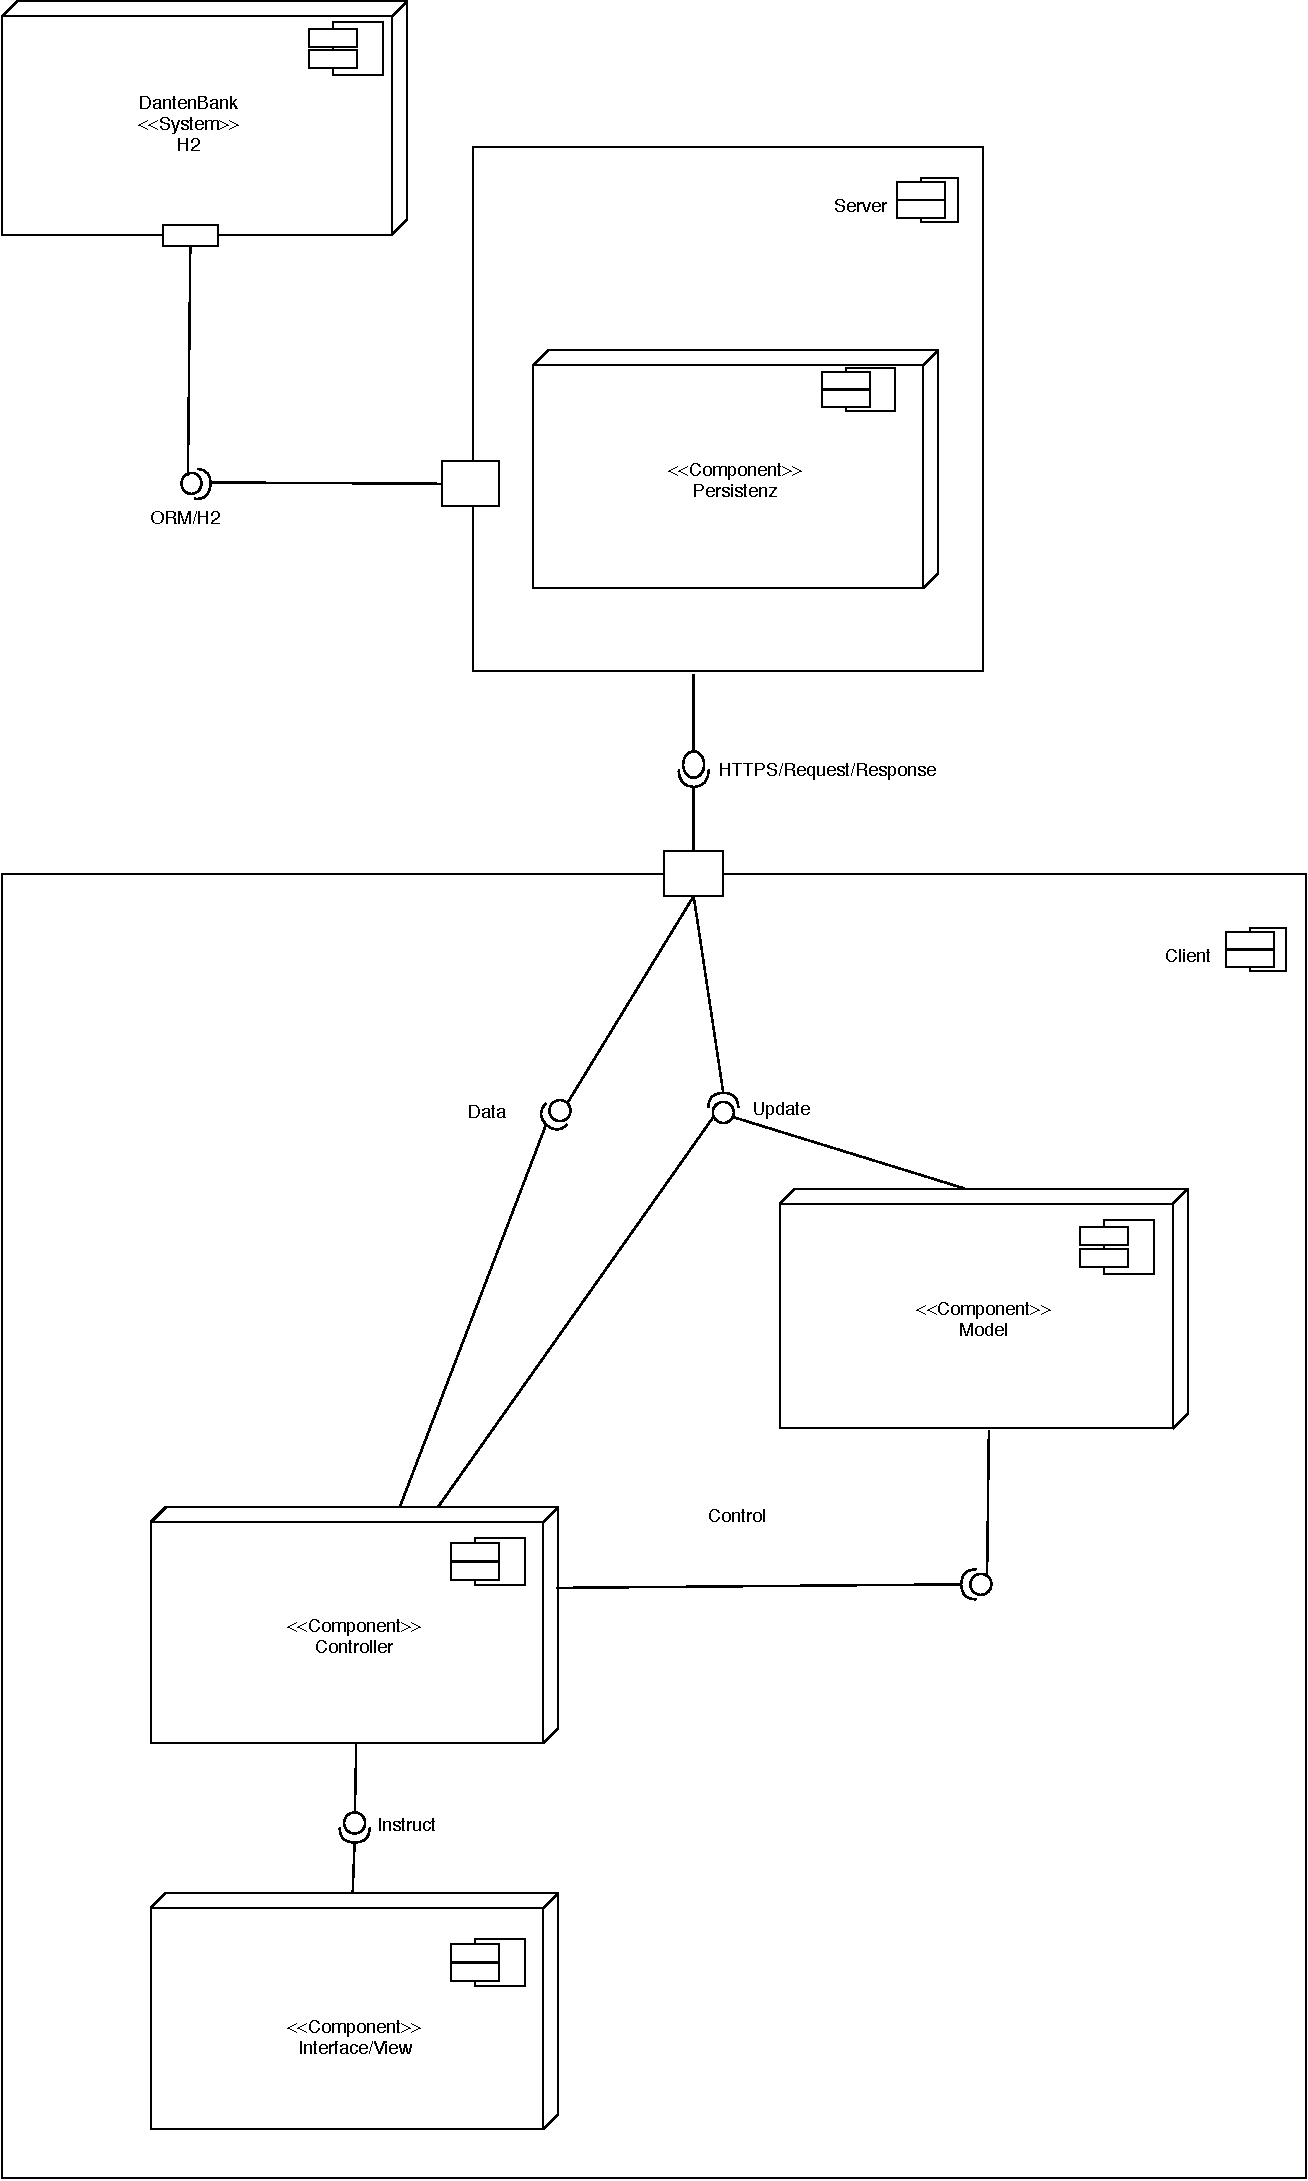
\includegraphics[width=340px]{UML/KonzeptionelleSicht.pdf}
  \caption{Die konzeptionelle Sicht}
  \label{fig:boat1}
\end{center}
\end{figure}


%%%%%%%%%%%%%%%%%%%%%%%%%%%%%%%%%%%%%%%%%%%%%%%%%%%%%%%%%%%%%%%%%%%%%%%%
\section{Pakete} \label{sec:pakete}

\subsection{Persistenz}

Das folgende Diagramm beschreibt unsere Persistenz. Persistenz Klassen werden dazu genutzt daten in der Datenbank zu speichern, verändern und löschen. Zu jedem im Spiel vorkommenden Objekt, bzw zu der Klasse aus dem das Objekt stammt, muss es ein so gennantes Data Access Object geben (kurz DAO), um diese in der Datenbank verwalten zu können.
Da viele von den DAOs die gleichen Funktionen haben, werden sie alle von einer Oberklasse ObjectDAO erben. ObjectDAO hat in sich drin auch eine Variable, welche die Verbundung zur Datenbank herstellt. Hiermit können so auch alle anderen DAOs auf die Datenbank zugreifen. Da wir ORMLite benutzen, wird auch jede unterklasse eine Variable des Typs Dao haben, welche zur abspeicherung der Daten verwendet wird. Um Daten abzuspeichern, wird die Methode persist(T) benutzt. Um daten zu löschen remove(T). Da manche Objekte in der Datenbank nicht verändert werden müssen (z.B. die Weltkarte), wird es keine Methode in der Oberklasse zum Updaten der Daten geben, sondern in jeder Unterklasse welche diese benötigt.

\begin{figure}[h!]
\begin{center}
  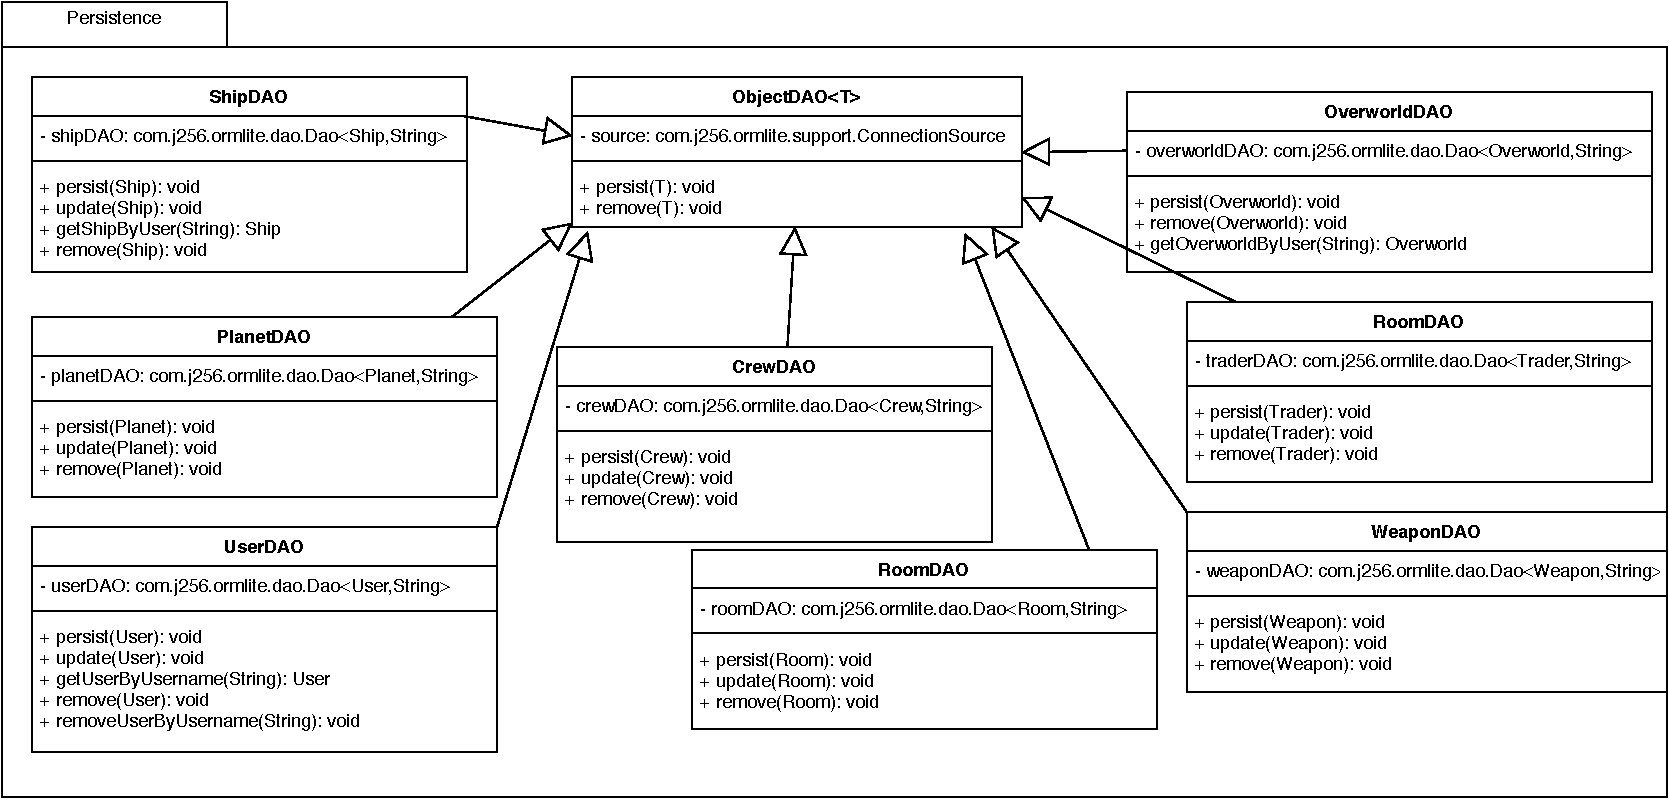
\includegraphics[width=\linewidth]{UML/PersistencePackage.pdf}
    \caption{Persistenz}
\end{center}
\end{figure}



%%%%%%%%%%%%%%%%%%%%%%%%%%%%%%%%%%%%%%%%%%%%%%%%%%%%%%%%%%%%%%%%%%%%%%%%
\section{Modulsicht} \label{sec:modulsicht}
{\itshape Diese Sicht beschreibt den statischen Aufbau des Systems mit Hilfe von
Modulen, Subsystemen, Schichten und Schnittstellen. Diese Sicht ist 
hierarchisch, d.\,h. Module werden in Teilmodule zerlegt. Die Zerlegung endet 
bei Modulen, die ein klar umrissenes Arbeitspaket für eine Person darstellen und
in einer Kalenderwoche implementiert werden können. Die Modulbeschreibung der 
Blätter dieser Hierarchie muss genau genug und ausreichend sein, um das Modul 
implementieren zu können.

Die Modulsicht wird durch {UML}-Paket- und Klassendiagramme visualisiert.

Die Module werden durch ihre Schnittstellen beschrieben.
Die Schnittstelle eines Moduls $M$ ist die Menge aller Annahmen, die andere 
Module über $M$ machen dürfen, bzw.\ jene Annahmen, die $M$ über seine 
verwendeten Module macht (bzw. seine Umgebung, wozu auch Speicher, Laufzeit 
etc.\ gehören).
Konkrete Implementierungen dieser Schnittstellen sind das Geheimnis des Moduls
und können vom Programmierer festgelegt werden. Sie sollen hier dementsprechend 
nicht beschrieben werden. 

Die Diagramme der Modulsicht sollten die zur Schnittstelle gehörenden Methoden
enthalten. Die Beschreibung der einzelnen Methoden (im Sinne der 
Schnittstellenbeschreibung) geschieht allerdings per Javadoc im zugehörigen 
Quelltext. Das bedeutet, dass Ihr für alle Eure Module Klassen, Interfaces und 
Pakete erstellt und sie mit den Methoden der Schnittstellen verseht. Natürlich 
noch ohne Methodenrümpfe bzw.\ mit minimalen Rümpfen. Dieses Vorgehen 
vereinfacht den Schnittstellenentwurf und stellt Konsistenz sicher.

Jeder Schnittstelle liegt ein Protokoll zugrunde. Das Protokoll beschreibt die 
Vor- und Nachbedingungen der Schnittstellenelemente. Dazu gehören die erlaubten
Reihenfolgen, in denen Methoden der Schnittstelle aufgerufen werden dürfen, 
sowie Annahmen über Eingabeparameter und Zusicherungen über Ausgabeparameter. 
Das Protokoll von Modulen wird in der Modulsicht beschrieben.
Dort, wo es sinnvoll ist, sollte es mit Hilfe von Zustands- oder 
Sequenzdiagrammen spezifiziert werden. Diese sind dann einzusetzen, wenn der
Text allein kein ausreichendes Verständnis vermittelt (insbesondere bei 
komplexen oder nicht offensichtlichen Zusammenhängen).

Der Bezug zur konzeptionellen Sicht muss klar ersichtlich sein. Im Zweifel 
sollte er explizit erklärt werden. Auch für diese Sicht muss die Entstehung 
anhand der Strategien erläutert werden.}

\subsection{Controller}
\begin{figure}[H]
\begin{center}
  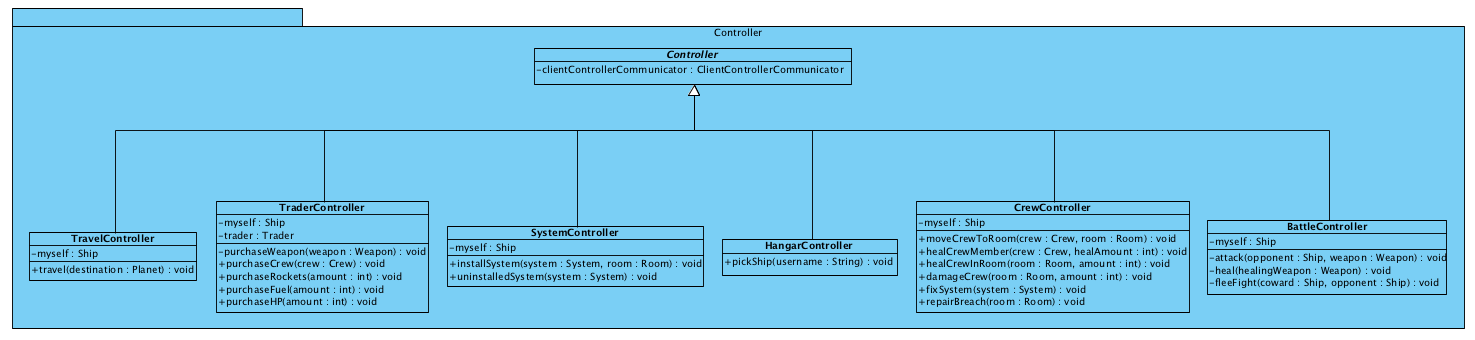
\includegraphics[width=\linewidth]{../GT_Modulsicht/src/Controllersicht.png}
    \caption{Controller}
\end{center}
\end{figure}

\subsection{View}
\begin{sidewaysfigure} 
\begin{center}
 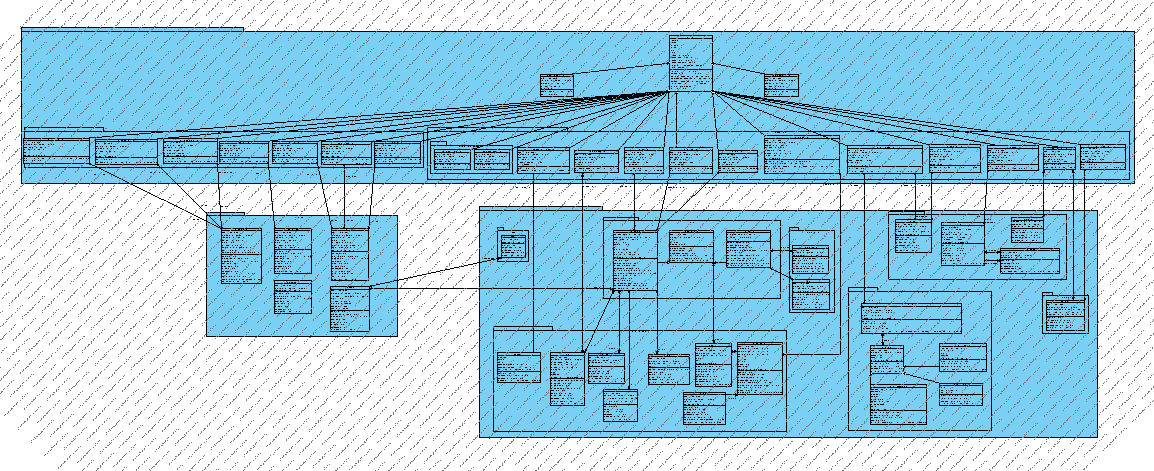
\includegraphics[width=\textwidth]{../GT_Modulsicht/src/View (2).pdf}
  \caption{Controller Sicht}
  \label{fig:boat1}
\end{center}
\end{sidewaysfigure}


\subsection{Communication Client}
\begin{figure}[H]
\begin{center}
  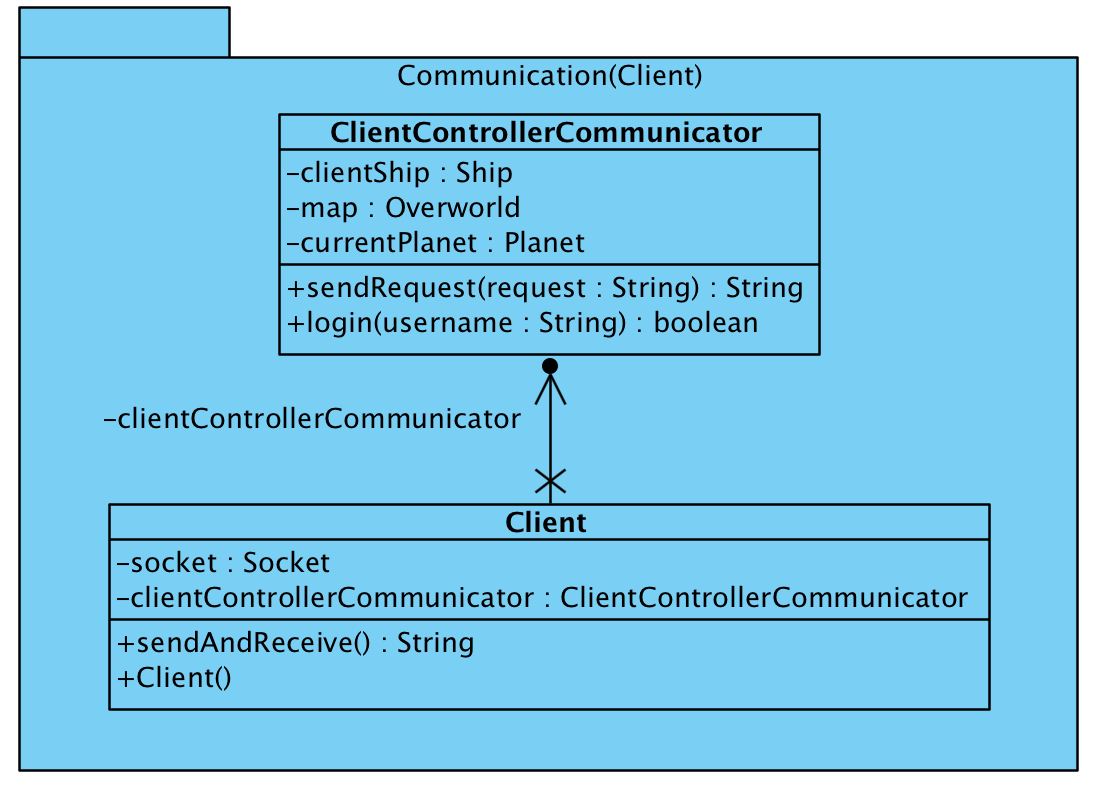
\includegraphics[width=\linewidth]{../GT_Modulsicht/src/CommClient.png}
    \caption{Das Datenmodell}
\end{center}
\end{figure}

\subsection{Communication Server}

\begin{figure}[H]
\begin{center}
  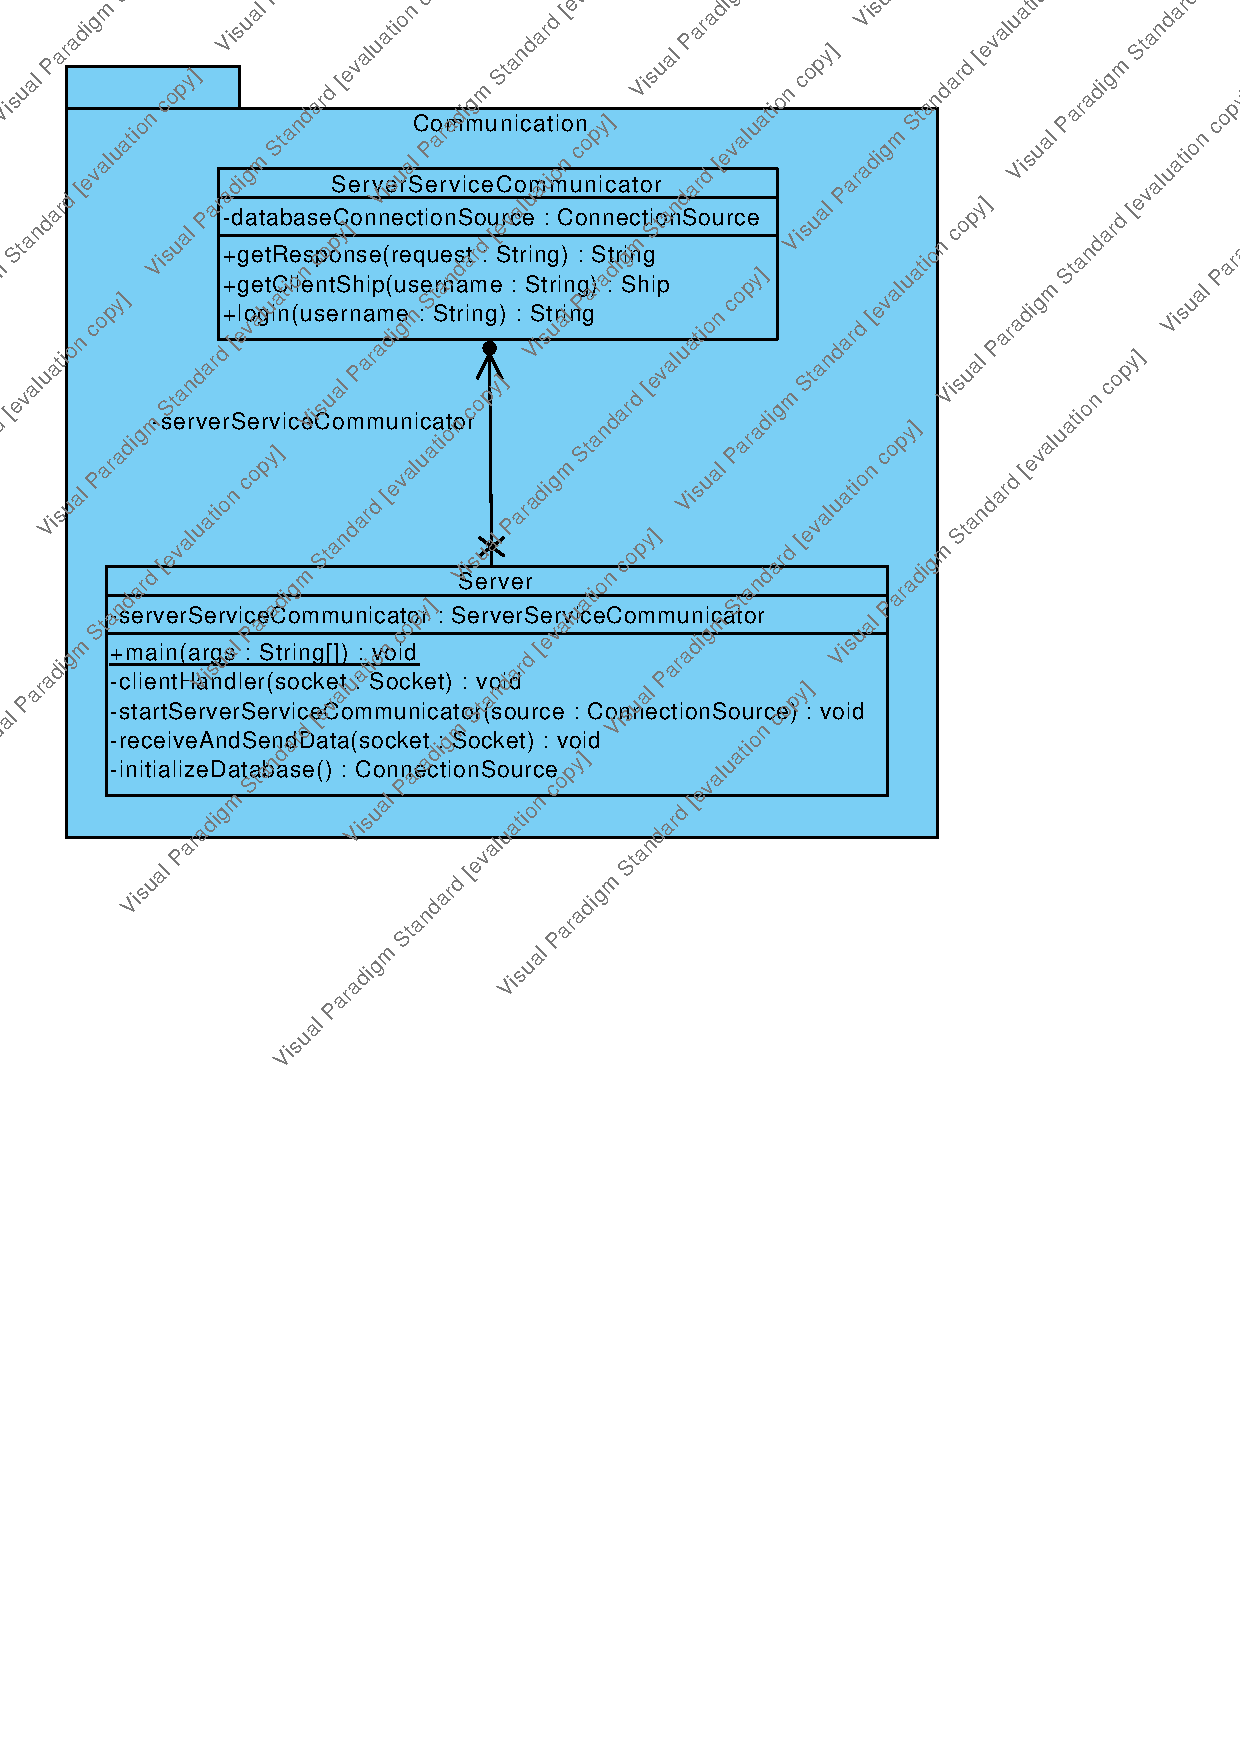
\includegraphics[width=\linewidth]{../GT_Modulsicht/src/CommServer.pdf}
    \caption{Das Datenmodell}
\end{center}
\end{figure}

\subsection{Service}

\begin{figure}[H]
\begin{center}
  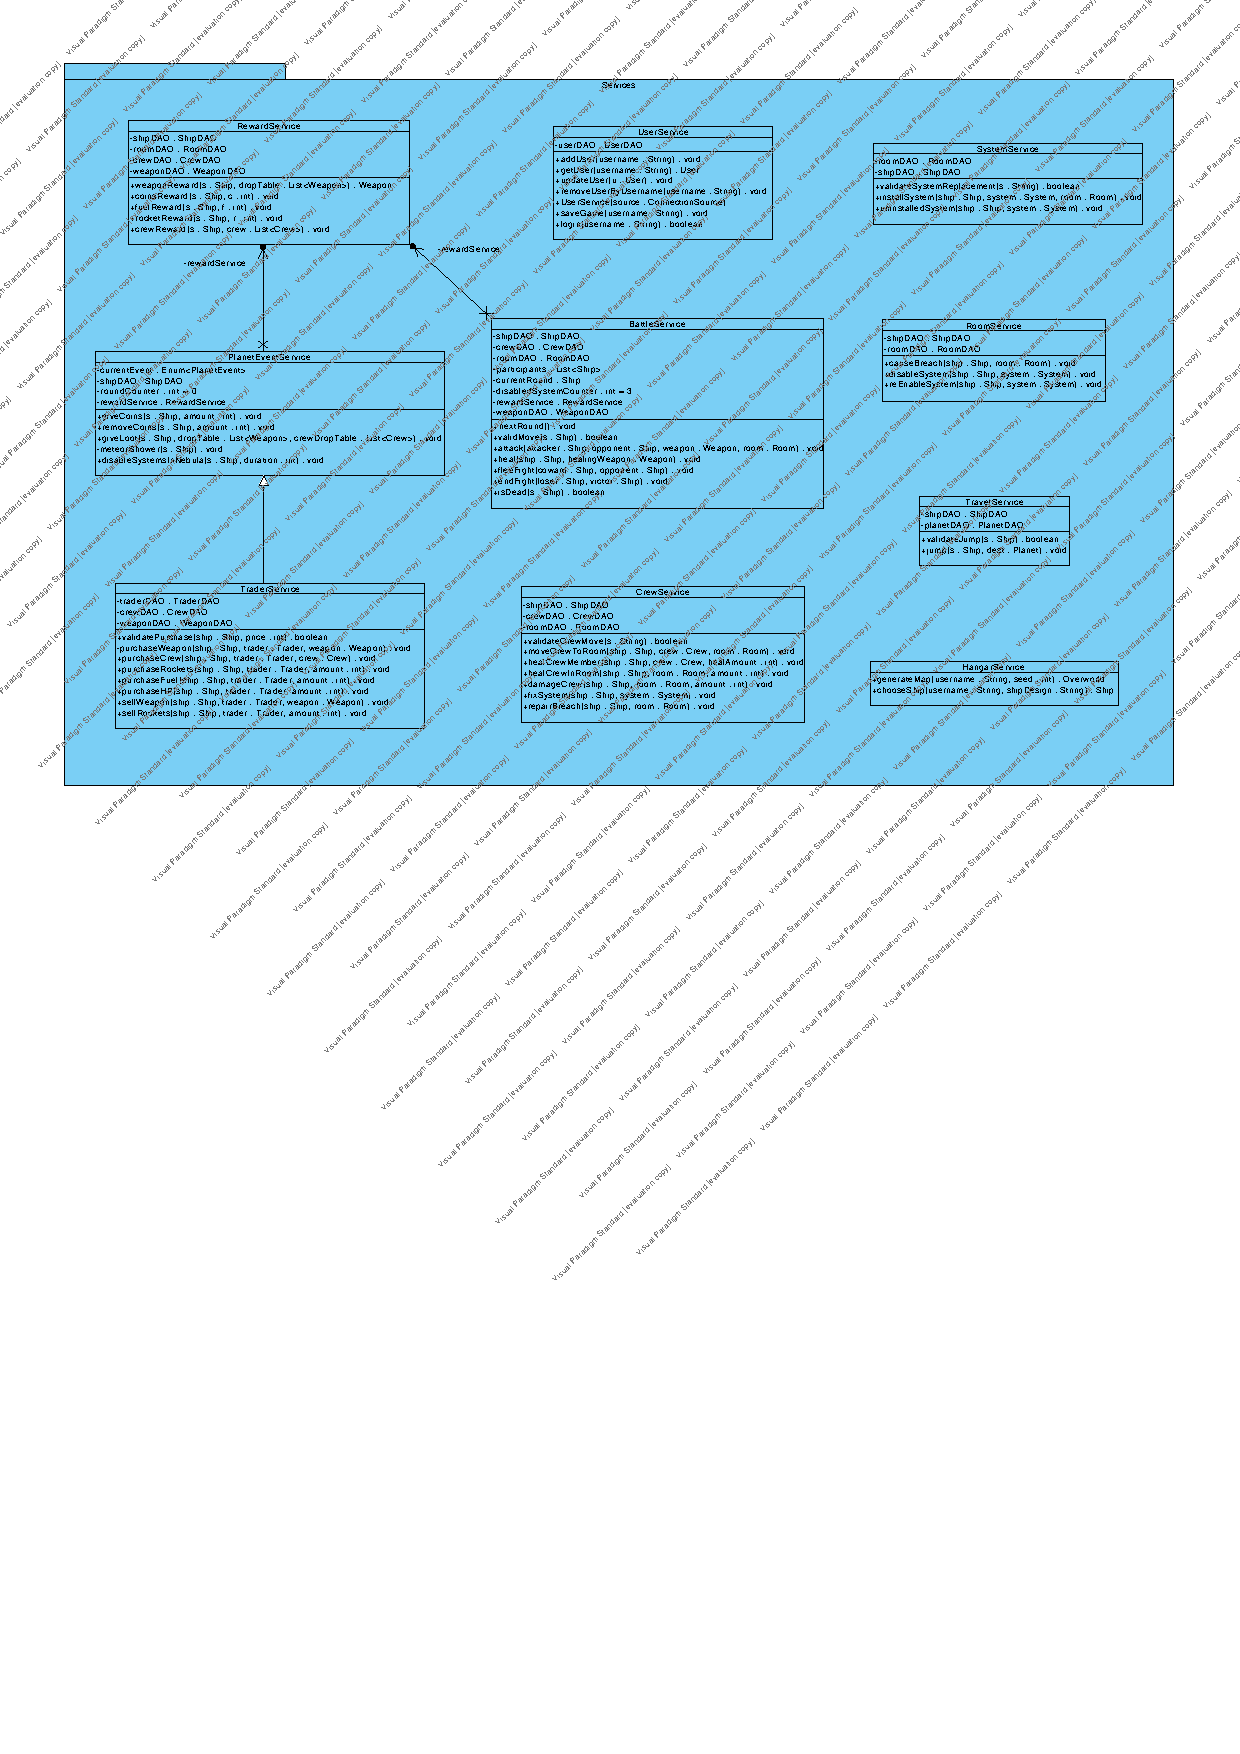
\includegraphics[width=\linewidth]{../GT_Modulsicht/src/Service.pdf}
    \caption{Das Datenmodell}
\end{center}
\end{figure}

\subsection{Model}

\begin{figure}[H]
\begin{center}
  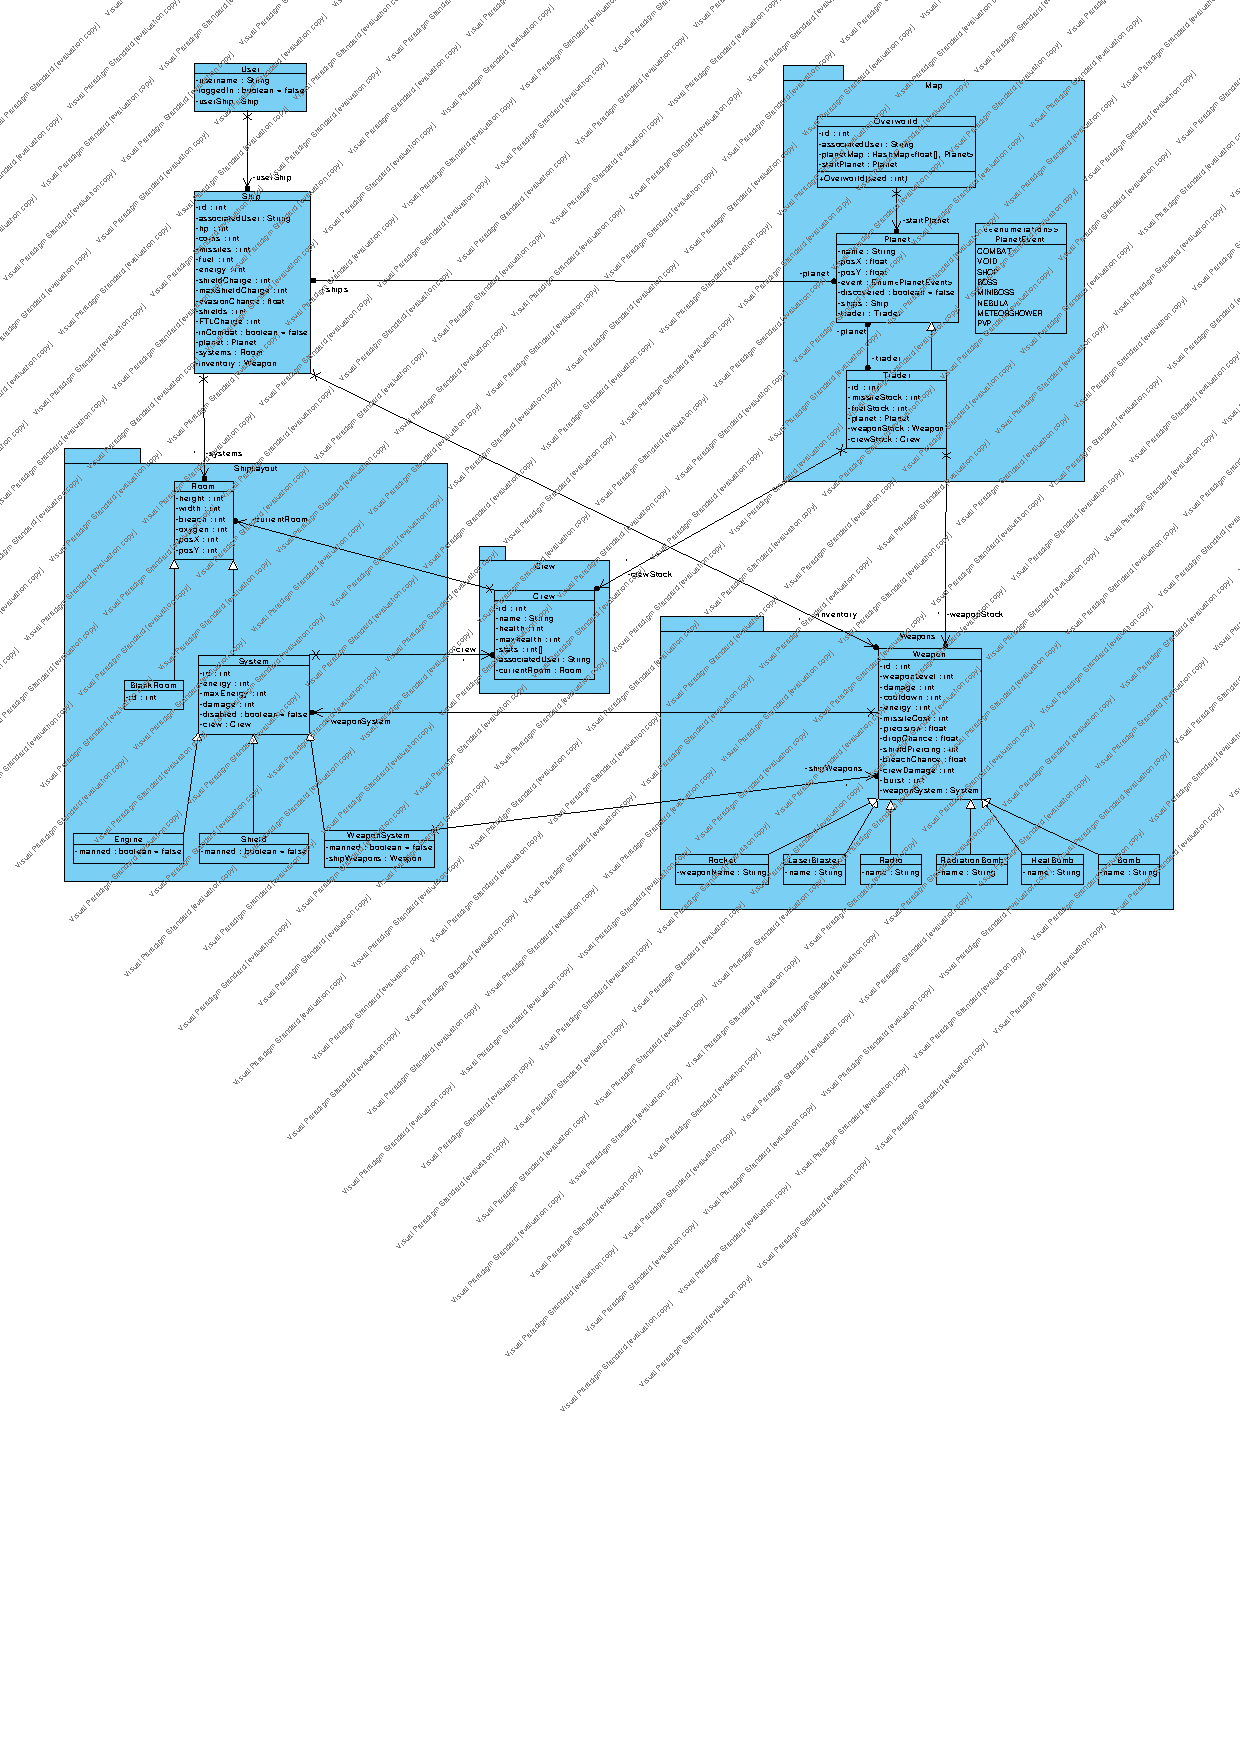
\includegraphics[width=\linewidth]{../GT_Modulsicht/src/Modelsicht.pdf}
    \caption{Das Datenmodell}
\end{center}
\end{figure}


%%%%%%%%%%%%%%%%%%%%%%%%%%%%%%%%%%%%%%%%%%%%%%%%%%%%%%%%%%%%%%%%%%%%%%%%
\section{Datensicht} \label{sec:datensicht}

{\itshape Hier wird das der Anwendung zugrundeliegende Datenmodell beschrieben. 
Hierzu werden neben einem erläuternden Text auch ein oder mehrere 
{UML}-Klassendiagramme verwendet. Das hier beschriebene Datenmodell wird u.\,a.\ 
jenes der Anforderungsspezifikation enthalten, allerdings mit 
implementierungsspezifischen Änderungen und Erweiterungen. Siehe die gesonderten
Hinweise.}

\textcolor{red}{TEXT}

Alle Spiel-relevanten Attribute sind in unserem Datenmodell in \textit{Ship} enthalten. Ein Schiff besteht aus mehreren Räumen , welche zum Teil leer sein können, aber auch wichtige Systeme beinhalten können. Damit realisieren wir die Strategie \textit{12.1} sowie die Strategien \textit{4.1} und \textit{4.2}.

Ein Raum kann wiederum unterschiedliche Systeme beherbergen, wie z.B. Schilde, Hüllen oder Antriebskomponenten, womit wir Strategie \textit{20.1-3} umsetzen können. Zusätzlich zu den oben genannten Systemen, gibt es noch eine Komponente \textit{WeaponSystem}, welche wiederum die \textit{abstract class Weapon} erweitert. Diese wiederum beinhaltet alle frei-schaltbaren Waffensysteme, womit wir die Strategien \textit{10.1-3} abdecken.

Des weiteren kann jeder \textit{Room}, bis zu 4 Crew Mitglieder gleichzeitig beherbergen. Womit wir die Strategie \textit{15.3} umsetzen. Zudem kann es vorkommen dass im Falle eines Angriffes/Zerstörung eines Raumes, Crewmitglieder mit einer gewissen Prozent-Chance schaden nehmen, oder sterben, womit wir die Strategien \textit{21.1 u. 21.2} erfüllen.

\begin{figure}[H]
\begin{center}
  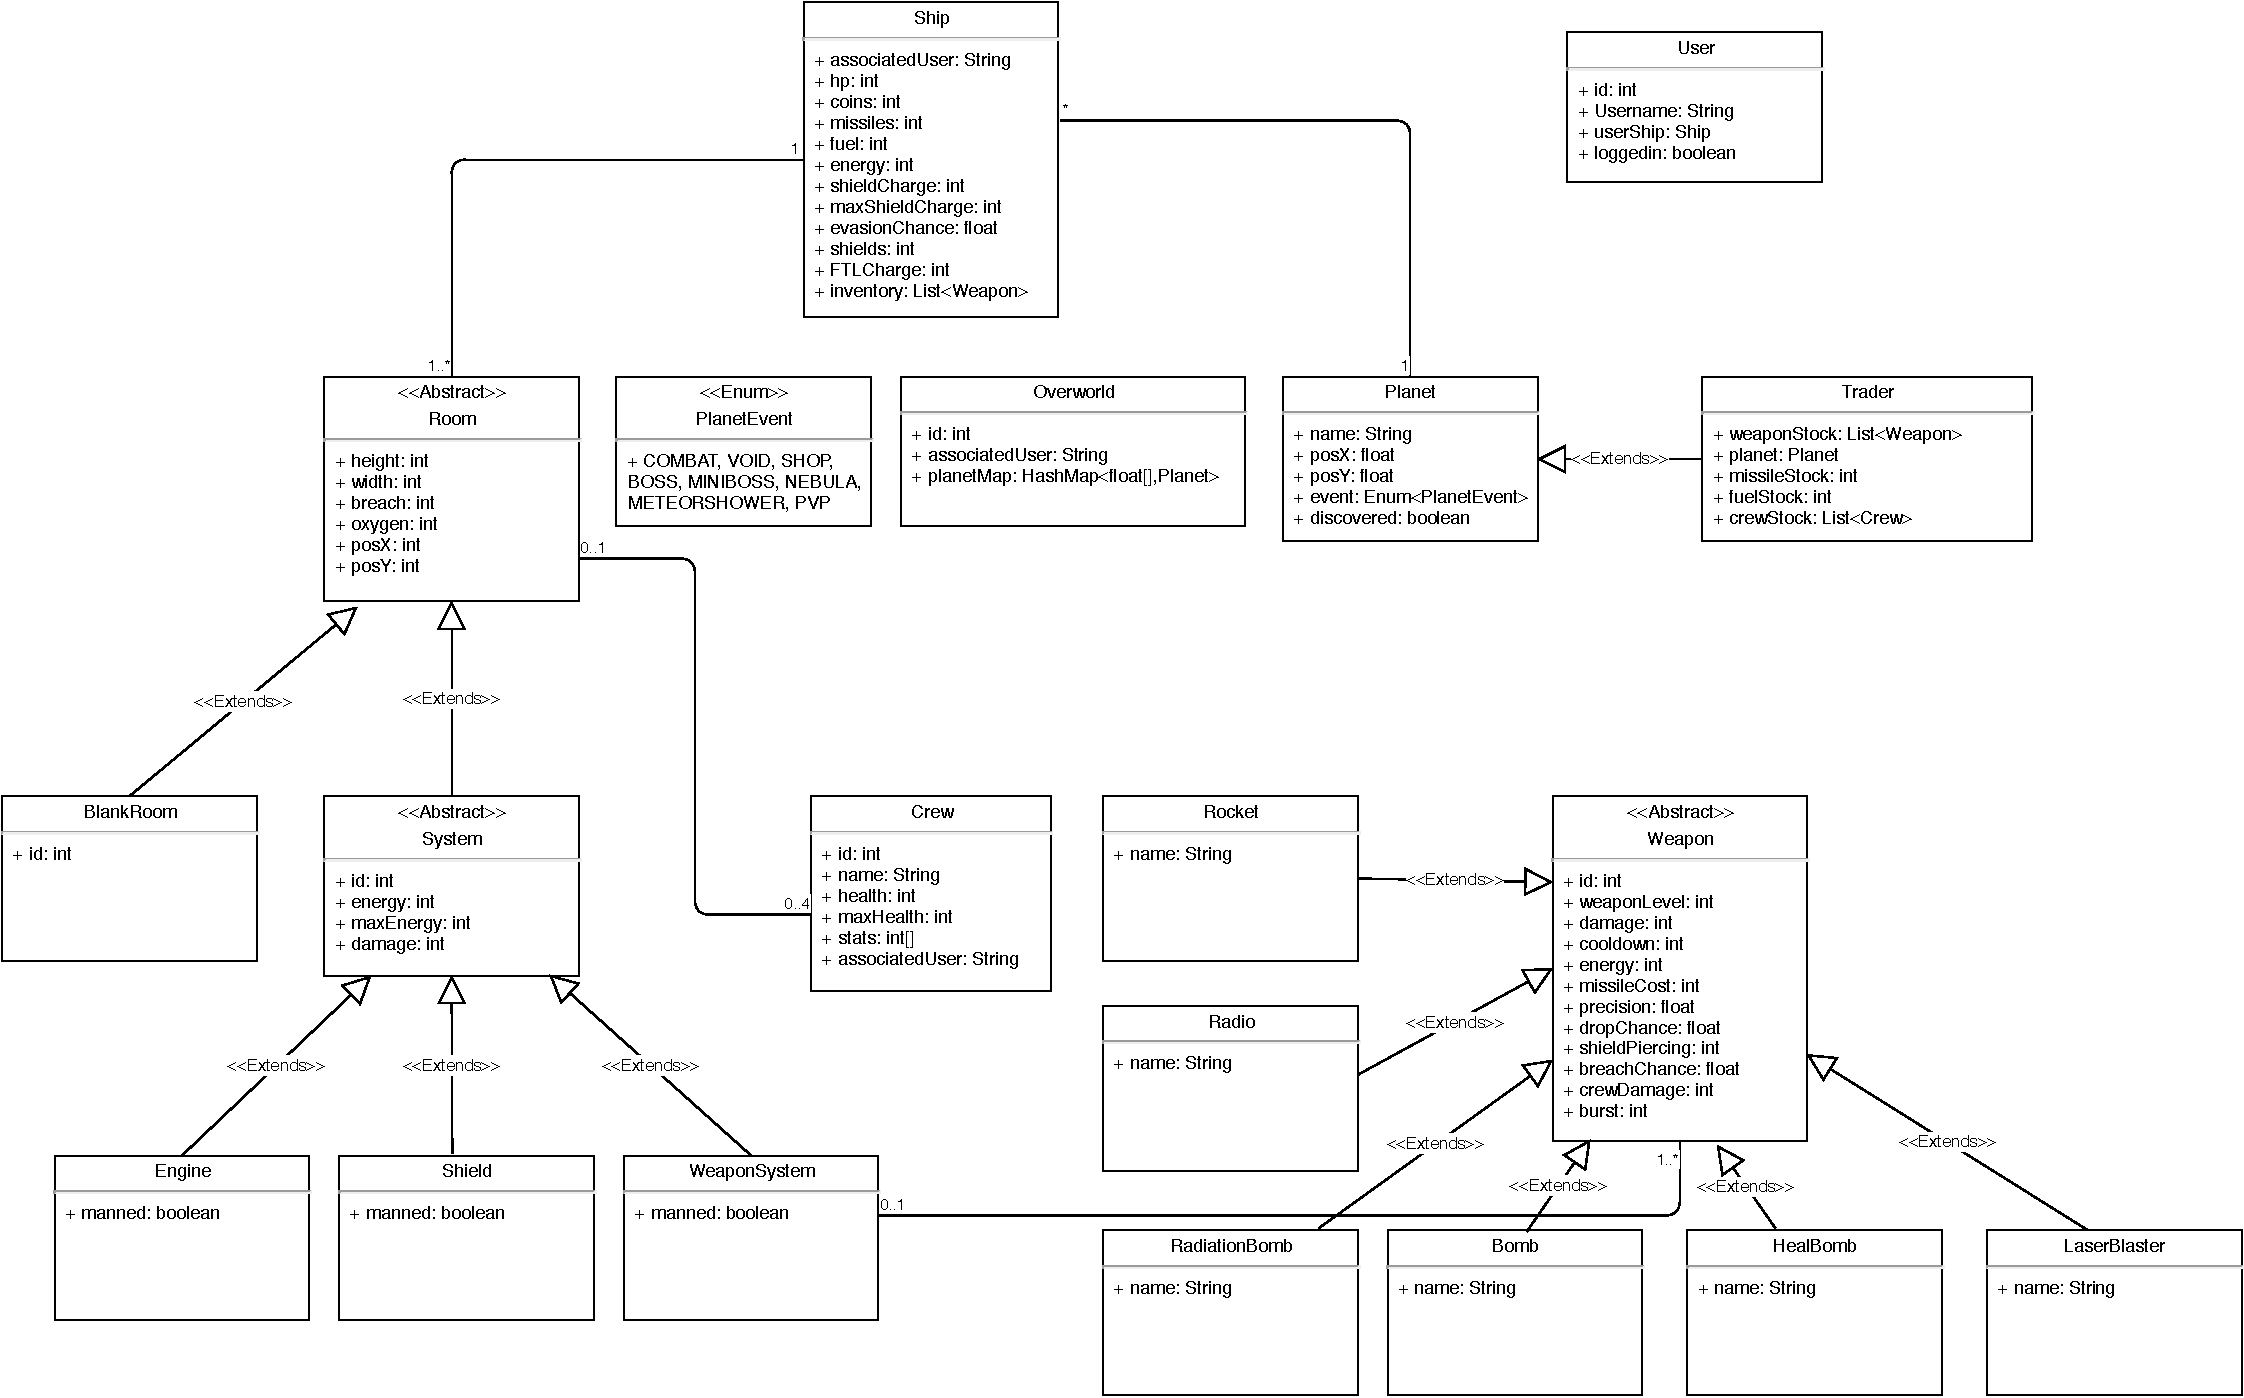
\includegraphics[width=\linewidth]{UML/Datenmodell.pdf}
    \caption{Das Datenmodell}
\end{center}
\end{figure}


%%%%%%%%%%%%%%%%%%%%%%%%%%%%%%%%%%%%%%%%%%%%%%%%%%%%%%%%%%%%%%%%%%%%%%%%
\section{Ausführungssicht} \label{sec:ausfuehrung}

%{\itshape Die Ausführungssicht beschreibt das Laufzeitverhalten. Hier werden die
%Laufzeitelemente aufgeführt und beschrieben, welche Module sie zur Ausführung 
%bringen. Ein Modul kann von mehreren Laufzeitelementen zur Laufzeit verwendet 
%werden. Die Ausführungssicht beschreibt darüber hinaus, welche Laufzeitelemente 
%spezifisch miteinander kommunizieren. Zudem wird bei verteilten Systemen 
%(z.\,B.\ Client-Server-Systeme) dargestellt, welche Module von welchen Prozessen
%auf welchen Rechnern ausgeführt werden.}

Im folgenden Schritt werden wir die Ausführungssicht erläutern. Es wird aufgezeigt, welche verschiedenen Geräte benötigt werden, welche Prozesse auf den Geräten jeweils laufen und welche Module dort enthalten sind. \\

\begin{figure}[H]
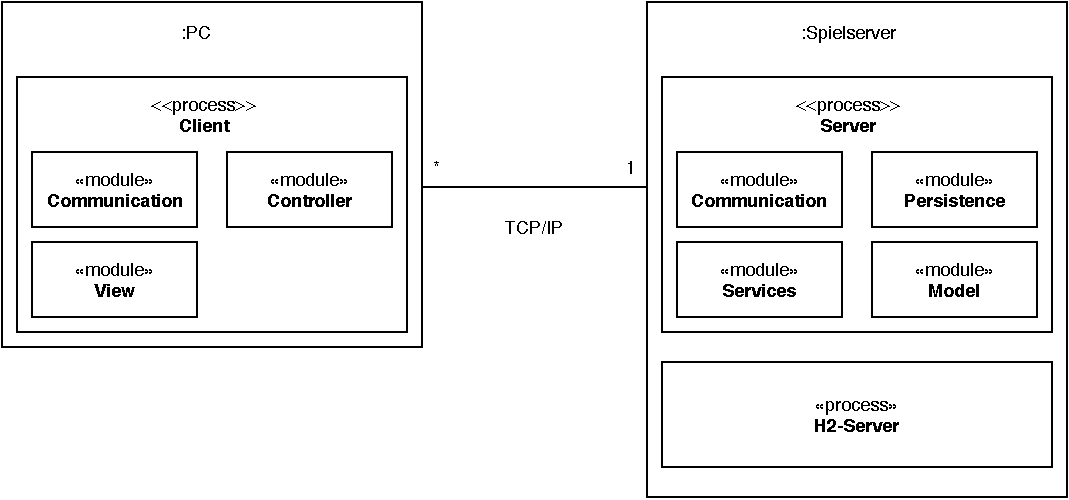
\includegraphics[width=\textwidth]{UML/Ausfuehrungssicht.pdf}
 \caption{Ausführungssicht}
\end{figure}

Die Ausführungssicht von unserem Spiel ist in der obigen Abbildung modelliert. Es gibt genau einen Anwendungsserver, auf dem unser System mit allen zugehörigen Modulen ausgeführt wird (Einflussfaktor T1.6). \\

Beliebig viele Benutzer können via TCP/IP auf den Spielserver zugreifen (mindestens zwei für eine Multiplayer-Session). Dies geschieht über die gestartete Spielanwendung auf dem Client-Rechner (hier wird Faktor P8.1 umgesetzt: Da die Spieler gegeneinander spielen sollen, müssen sie sich auf dem gleichen Server befinden). In diesem Prozess läuft die Kommunikation über Communication Module auf Client und Server Seite. \\

Auf dem Anwendunsserver laufen sowohl das System, als auch eine Instanz der H2-Datenbank (wodurch Strategie 3.1 umgesetzt wird).
Das Modul Persistence kommuniziert mit der Datenbank über ORM-Lite.  \\ 

%%STRATEGIEN




%%%%%%%%%%%%%%%%%%%%%%%%%%%%%%%%%%%%%%%%%%%%%%%%%%%%%%%%%%%%%%%%%%%%%%%%
\section{Zusammenhänge zwischen Anwendungsfällen und Architektur}
\sectionmark{Zusammenhänge AF u. Architektur} \label{sec:anwendungsfaelle}

\subsection{Server-Client-Kommunikation}

\begin{figure}[H]
\begin{center}
  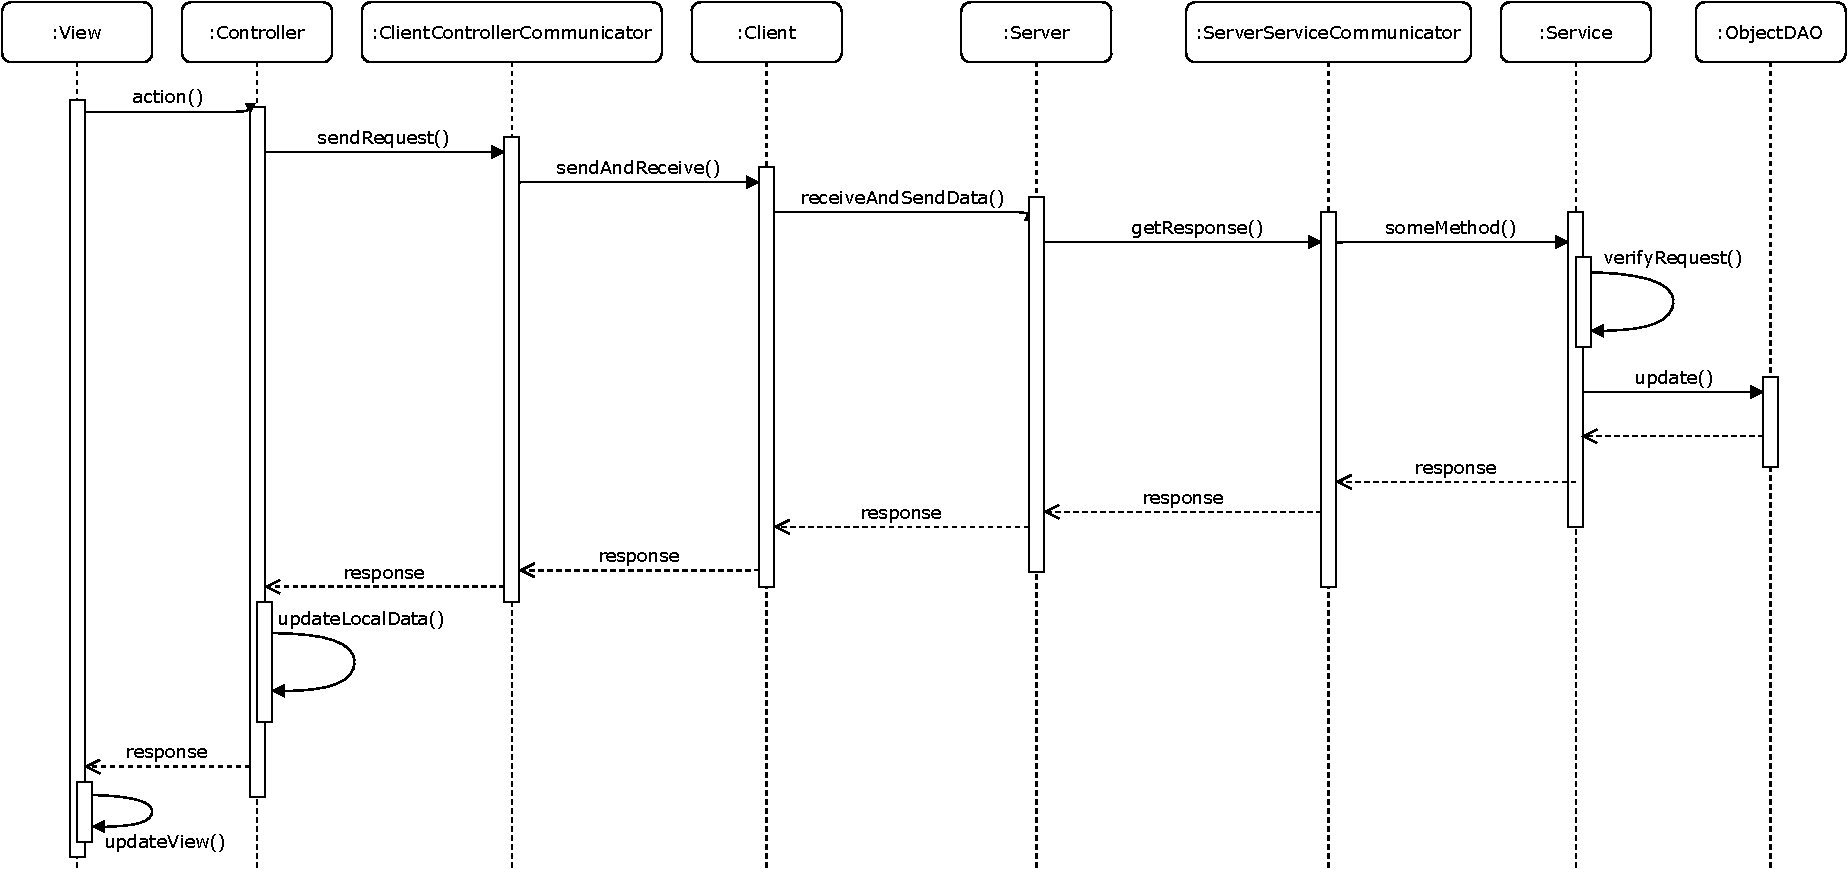
\includegraphics[width=\linewidth]{UML/Server_client_Sequenzdiagramm.pdf}
\end{center}
\end{figure}

Das obige Diagramm beschreibt abstrakt wie der Game-Client eine Aktion ausführen möchte, und wie diese vom Server empfangen und bearbeitet wird.
Der Client möchte z.B. eine Angriffsaktion ausführen, diese muss allerdings erst vom Server überprüft werden. Der Benutzer clickt in seinem View auf einen Knopf, welcher die 
korrekte Methode aus dem korrekten Controller ausführt, welche zu dieser Aktion gehört. (Einen konkreten Fall werden wir im nächsten Diagramm vorstellen)
Der Controller erstellt ein neues Request welches dann an den ClientControllerCommunicator weitergegeben wird, welcher es dann an die Netwerkschnittstelle Client weiterleitet. Diese Netzwerkschnittstelle schickt dann dieses Request an den Server, wo sie dann von der Schnittstelle des Servers akzeptiert wird. Der Server empfängt das Request und gibt es an seinen ServerServiceCommunicator weiter, welches das Request dann an das korrekte Service weiterleitet. Das Service prüft ob das Request valide ist. Ist dieses der Fall, so wird die Logik des Requests ausgeführt und die Daten in der Datenbank angepasst. Nach der Bearbeitung der Daten wird ein Response an den ServerServiceCommunicator gegeben. War das Request nicht valide, so wird auch dies dem ServerServiceCommunicator mitgeteilt. Dieser leitet dann das Response das er bekommen hat weiter an die Server Schnittstelle, welches die Daten dann zum Client schickt. Der Client empfängt das Response und gibt es seinem ClientControllerCommunicator, welcher es auch wiederrum an den korrekten Controller weiterleitet. Der Controller führt nun seine Logik aus, passt seine lokalen Daten an und gibt dem View bescheidt, so dass dieser sich auch aktualisiert.

\subsection{Angriff}

\begin{figure}[H]
\begin{center}
  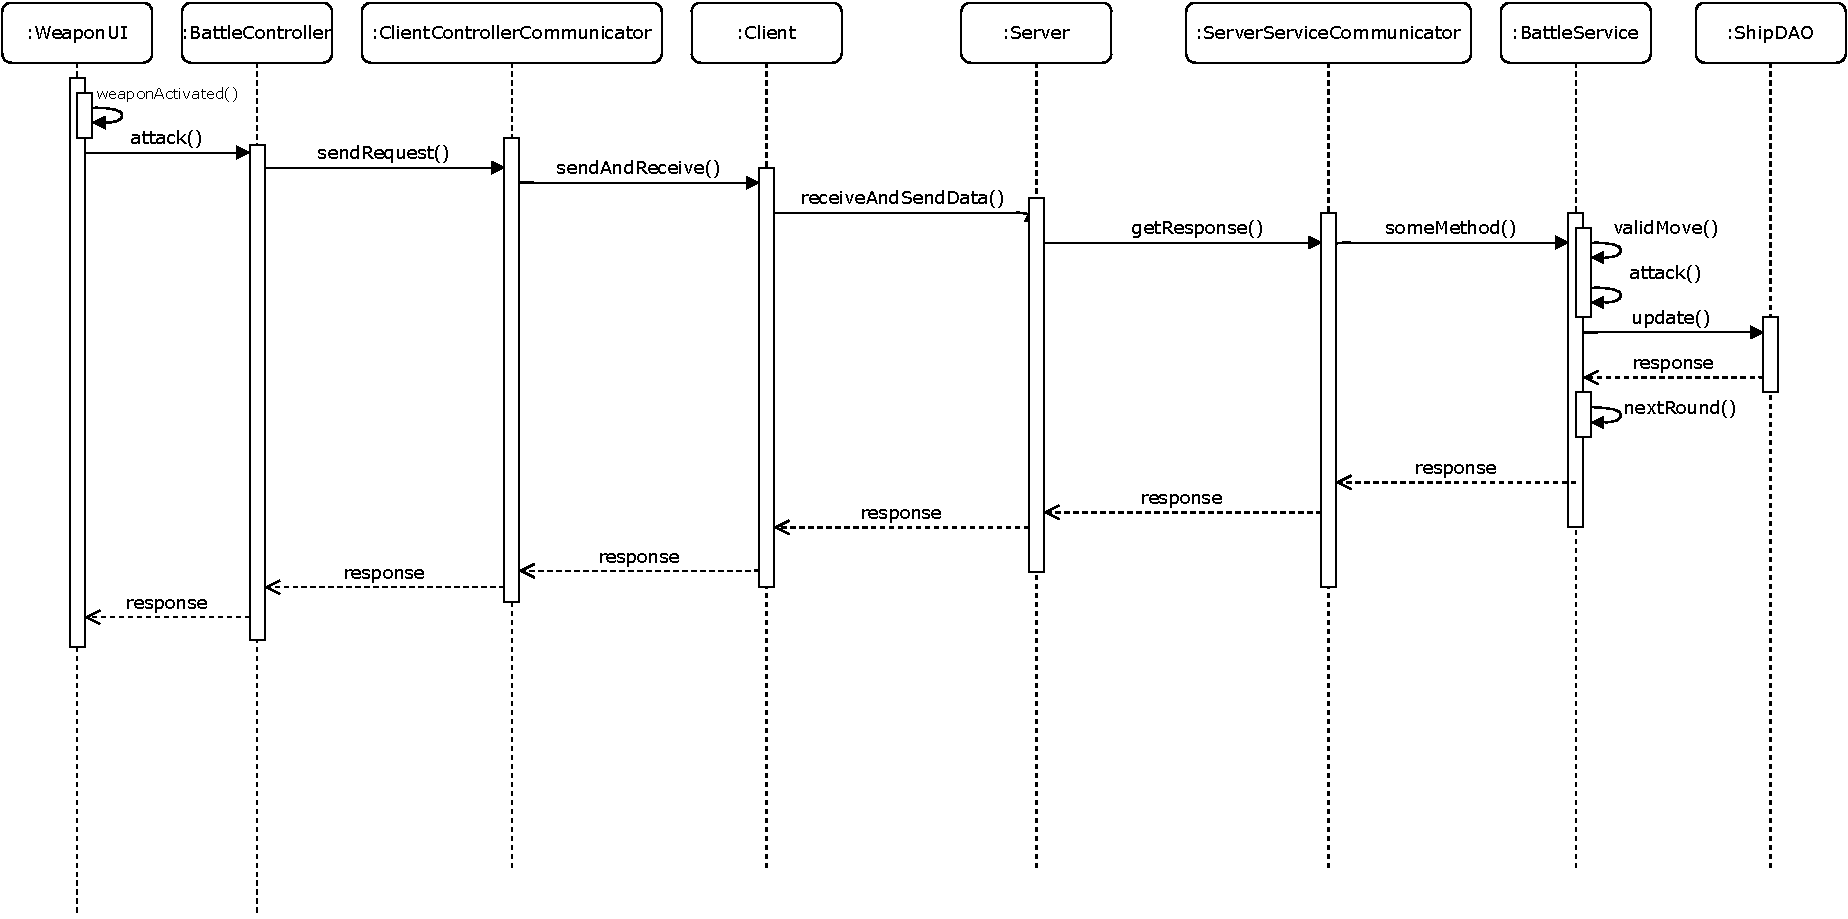
\includegraphics[width=\linewidth]{UML/Sequenz-Attack.pdf}
\end{center}
\end{figure}

Dieses Diagramm beschreibt nun eine Attack-Sequenz basierend auf dem vorherigem abstrakten Diagramm. In diesem Fall wird in der WeaponUI eine Waffe durch Mausclick ausgewählt, und dann der Raum auf dem Gegnerschiff welcher angegriffen werden soll. Dann wird dieses als Attack-Request weitergegeben an den ClientControllerCommunicator, welcher es wiederrum an die Netzwerkschnittstelle des Clients weiterleitet. Das Request wird dann durch diese Schnittstelle an den Server geschickt. Der Server empfängt das Request und gibt es an seinen ServerServiceCommunicator, welcher dann den AttackService wählt und ihm das Request weiterleitet. Dieser überprüft dann mittels ValidMove ob das Angriffskommando valide ist oder nicht. Wenn es das ist, so wird die Logik ausgeführt, und das Gegnerschiff in der Datenbank aktualisiert. Dann wird der jetzige Spieler weitergesetzt (wer dran ist). Dann wird ein Response als neue Schiffsobjekte an den ServerServiceCommunicator gegeben, welcher es wieder an die Servernetzwerkschnittstelle gibt. Das Response wird dann zum Client übertragen, und dort an den ClientControllerCommunicator gegeben. Dieser teilt das Ergebnis dem Controller mit (gleiche Methode, da diese noch auf den Response wartet). Dann werden dort die lokalen Daten durch die vom Server bekommenen Daten ersetzt. Der View wartete bis jetzt noch auf ein Ergebnis welches er nun bekommt, wodurch auch er sich aktualisiert.


\subsection{Login}

\begin{figure}[H]
\begin{center}
  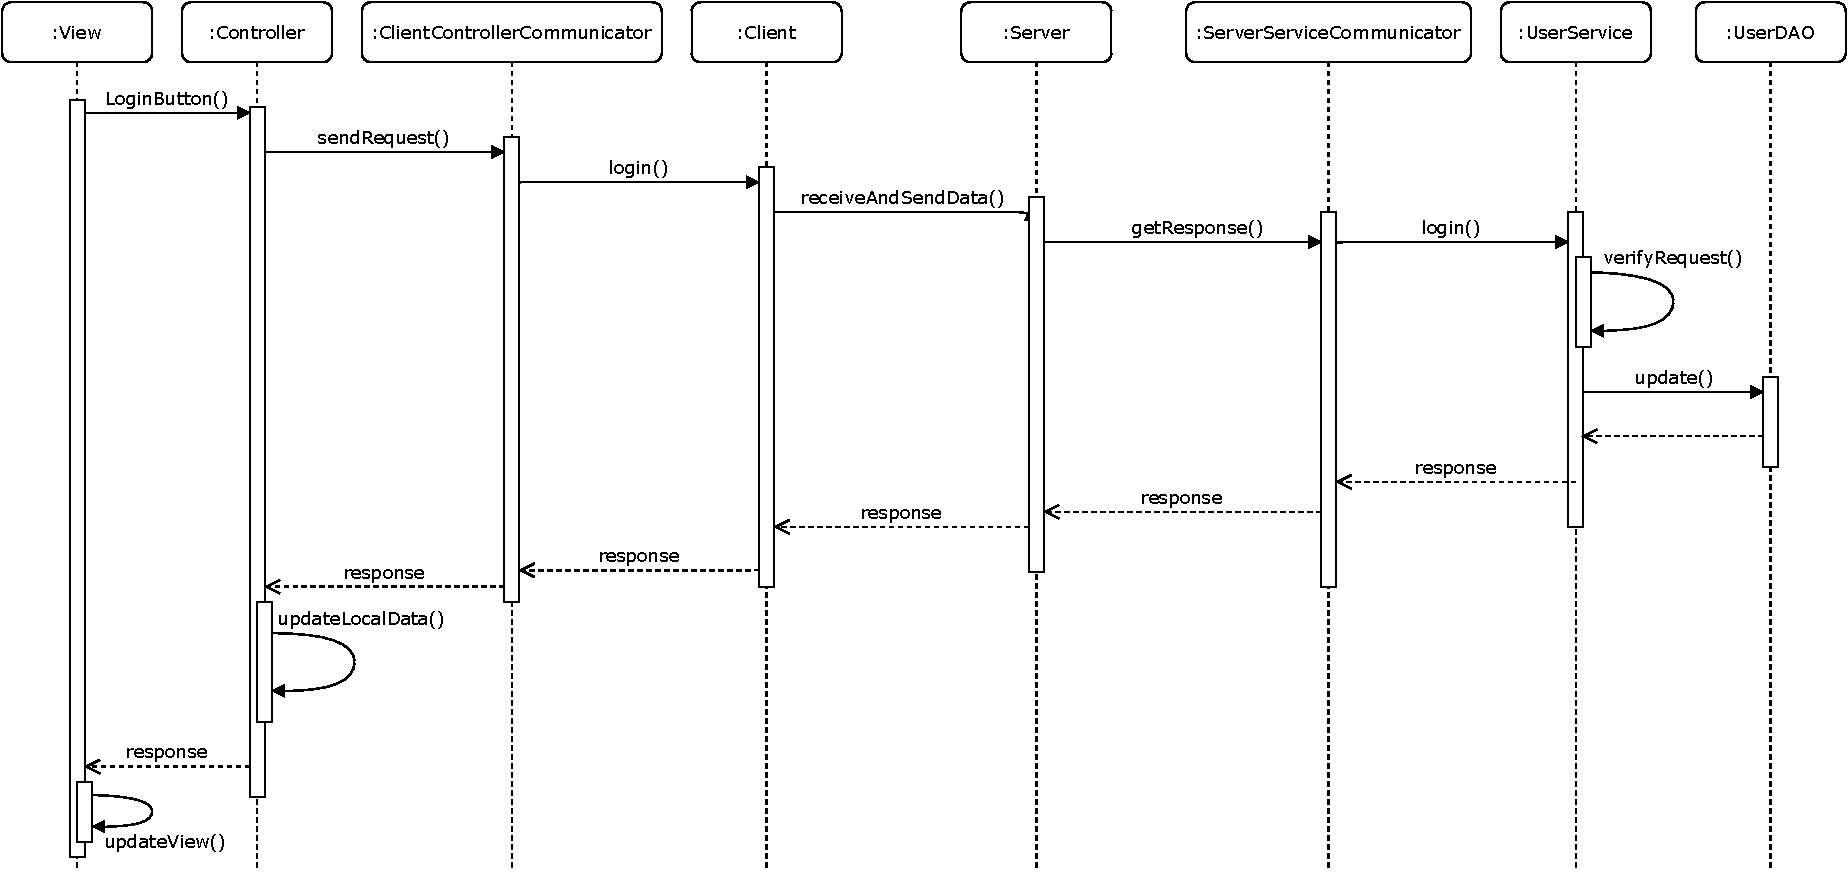
\includegraphics[width=\linewidth]{UML/Sequenz-Client-login.pdf}
\end{center}
\end{figure}

Das hier gezeigte Diagramm zeigt den Login eines Spielers, dabei wird im View erstmals der \textit{LoginButton()} durch einen Mausklick ausgewählt und durch den Controller wird eine Request an den \textit{ClientControllerCommunicator} gesendet, dieser wiederum führt die Methode \textit{login()} aus, welche dann einen LoginRequest über die Methode \textit{receiveAndSendData} an den Server sendet. Auf der Server Seite wird nun die Methode \textit{getResponse()} aufgerufen, welche im \textit{UserService} die Logik und die Verifizierung des Logins mithilfe des \textit{usernames} ausführt. Wenn nun der Login genehmigt wurde durch den Service, so wird der Request verifiziert und die \textit{UserDao} wird geupdated. Nun geht die \textit{Response} über die gleichnamigen Methoden zurück zum Client welcher die Response weitergibt an den Controller. Der Controller updated die Lokalen Daten und übergibt die aktualisierten Daten an den View. Nun ist der User eingeloggt und kann der Session beitreten.


%%%%%%%%%%%%%%%%%%%%%%%%%%%%%%%%%%%%%%%%%%%%%%%%%%%%%%%%%%%%%%%%%%%%%%%%
\section{Evolution} \label{sec:evolution}


In folgendem Abschnitt behandeln wir mögliche Weiterentwicklungen für unsere Software. Es werden die Ideen und notwendige Veränderungen an der Architektur dargestellt.


\subsection{Fraktionskampf}
Drei Fraktionen treten auf einer sehr großen Map im Mehrspielermodus gegeneinander an. Jede Fraktion hat ein Hauptquartier von dem aus alle Spieler starten. Die Karte besteht aus vielen großen und kleinen Kontrollstationen, welche durch kleinere Systeme dargestellt werden, welche zu Beginn der Runde neutral sind und einfach eingenommen werden können. 
Im weiteren Verlauf müssen die Fraktionen im Kampf um mehr Ressourcen und Gebiete aufeinandertreffen und in mehreren Runden um die Kontrollpunkte kämpfen, dabei sollen Große Kontrollpunkte/Stationen mehrere Runden benötigen, um diese einnehmen zu können. Größere Stationen ermöglichen mehr Boni und Ressourcen, sowie eine größere Gebietskontrolle. Kleinere Stationen decken kleine Gebiete ab und sind schneller einzunehmen. Dabei ist es das Ziel der Angreifenden Fraktion, die Station direkt anzugreifen, zu beschädigen und letzendlich, wenn die Waffen der Station/Schilde ausgeschaltet sind, sie zu übernehmen. Das jeweilige Gebiet wird der jeweiligen Fraktion gutschrieben und die Boni werden angewandt. 
Dies soll verhindert werden können, indem Angreifende Schiffe einen Timer auslösen, welcher für die Verteidiger einsehbar ist. Dieser Timer dient für die Verteidiger dazu, zur Station zurückzukehren und das angreifende Schiff in 1vs1 Kämpfen abzufangen und aufzuhalten, bevor dieses der Station schaden kann.
 Falls also ein angreifendes Schiff nicht abgefangen werden kann, weil zu wenige oder keine Verteidiger mehr vorhanden sind, oder sich nicht in der Nähe des Systems befinden, so soll der Angreifer der Station schaden können. Dies soll je nach Stärke und Ausbau der Verteidungsanlagen länger dauern und mehr Teamwork benötigen, als Stationen die kaum Ausgebaut wurden.
 Das Balancing soll dabei folgendermaßen funktionieren: Die Fraktionen müssen Schlüsselrouten und deren Stationen gut verteidigen und ausbauen, zudem die Spieler auf die Karte und auf einzelne \glqq Missionen\grqq{} aufteilen, um effektiv weitere Gebiete für sich zu gewinnen. Einzelne Schiffe sollen zudem keine großen Stationen alleine einnehmen können, damit keine Alleingänge und \glqq Schwarm-Taktiken\grqq{} möglich sind, weil es nicht möglich sein soll mit einzelnen Schiffen ganze Systeme erobern zu können und die eigene Flotte so aufzuteilen dass der Gegner diese einzelnen Schiffe nicht aufhalten kann. 
 Das Balancing ist also stark davon abhängig, wie viel Team-Kommunikation zwischen den Spielern stattfindet und wie deren taktisches Know-How ist. 
 Die Schiffe soll man zudem immer umrüsten können und auf die jeweiligen Abwehr/Waffensysteme der Gegner anpassen können. Dieses Umrüsten soll nur bei eigenen Stationen möglich sein und nicht überall. 
 Änderungen an der Architektur wären hierbei, die Erweiterung des Servers, sodass er mit vielen verschiedenen Spieler-Eingaben, dem Managment der Spieler in den verschiedenen Fraktionen, sowie deren Auswirkung auf die Spielwelt klarkommt. Es muss außerdem eine große Spielwelt erstellt werden, welche in Sektoren, die eingenommen werden können, aufgeteilt wird. Die Datenbank muss diese zusätzlichen Daten verarbeiten und den Spielern auf der Karte immer eine aktuelle Version des Zustands von Stationen, sowie die Positionen von nahen Feindschiffen anzeigen können. 




\subsection{Kreativmodus (Sandbox)}
{
Der Kreativmodus soll ein eigener Solomodus werden, indem der Spieler sein Schiff nach freiem Belieben aus einer Liste aller im Spiel enthaltenen Eigenschaften für ein Schiff erstellen kann. Zunächst wählt der Spieler ein Raumschifflayout, anschließend trifft er eine Auswahl für Systeme, eine Auswahl für das Level der Systeme, eine Auswahl an Waffen und deren Level und eine Auswahl an Crew, wobei man bei jedem Crewmitglied die Spezies (und die damit verbundene Spezialfähigkeit) und die Level individuell einstellen kann. 
Das Schiff kann im Kreativmodus als (benannte) Vorlage gespeichert werden, um es bei zukünftigen Testspielen selbst oder als Gegner zu verwenden.

Hat man dann seine eigene Ausrüstung nach seinem Belieben ausgewählt, kann man damit nun ein Testspiel starten (Hierbei werden keine Errungenschaften o.Ä. freigeschaltet). Ein Testspiel verhält sich genau so wie ein normales Spiel, nur dass man nichts freischalten kann und somit wird sich dieses Testspiel, wie auch alles andere im Kreativmodus, nicht auf den normalen Spielfortschritt auswirken. 

Alternativ kann man auch einen Testkampf (Sandbox)(gegen einen zufälligen, ähnlich angepassten Gegner oder gegen einen selbst vorkonfigurierten Gegner) starten. Hier wird man also in einen Schlachtfeld gespawnt, kann sich auf den Kampf vorbereiten und hat dann Buttons, mit dem man Gegnerische Schiffe spawnen kann. Man kann nach eigenem Belieben ein oder mehrere Schiffe spawnen, diese aus Vorlagen oder zufälligen Vorlagen spawnen, und man kann für jeden Gegner eine Schwierigkeit wählen. Es gibt kein Ende, sodass man sobald man keine Lust mehr hat, den Testkampf einfach über einen Button beenden kann. 

\textit{Sinn des Modus:}
Man kann neue Setups testen, auf die man hin arbeiten will, oder man lässt seinen Frust an vergleichsweise schlechten Gegnern aus, welche man mit viel zu übertriebenen Waffen zerschmettert. Wie der Name schon sagt, soll der Kreativität des Spielers (fast) keine Grenzen gesetzt werden.

An der Architektur muss soweit nichts großartig verändert werden, da man ein Testspiel genauso auch im richtigen Modus spielen könnte. Einzig die Errungenschaften und Freischaltungen müssten für den Modus gesperrt werden. Um die Kampf Sandbox zu erstellen, könnte in der Architektur eine neue Sicht erstellt werden, welche nicht eine Karte wie normale Spiele beinhaltet, sondern nur das Kampffeld.  Man müsste im Model verändern, dass Kämpfe mit mehr als 2 Raumschiffen erlaubt sind, sodass man nicht nur Kämpfe gegen einen Gegner führen kann. 

}

\subsection{CO-OP-Modus}
{
Der CO-OP-Modus soll so wie der Einzelspielermodus sein. Das Ziel ist es, Ausrüstung zu sammeln, indem man computergesteuerte Raumschiffe zerstört oder die Zufallsereignisse absolviert. Mit dieser Ausrüstung kann man dann am Ende den Endboss besiegen. Der Unterschied zum Einzelspielermodus ist der, dass man zu zweit über einen ähnlich zum Mehrspielermodus aufgebauten Server spielen kann und alle Gegner zusammen angreifen und besiegen kann, aber nicht muss. Es soll auch möglich sein, dass die Spieler an unterschiedlichen Orten spielen. Außerdem könnte man einen Handel zwischen den beiden Spielern erlauben, sodass man die erkämpfte Ausrüstung untereinander tauschen kann.

In der Architektur muss ein neuer Modus für den Server erstellt werden, sodass kein PVP mehr möglich ist. Stattdessen müssen im Model Kämpfe mit drei Schiffen erlaubt werden. Außerdem müsste noch die Mechanik zum handeln/tauschen implementiert werden. Dies könnte ähnlich zum Shop implementiert werden.
}



\end{document}

%%% Local Variables: 
%%% mode: latex
%%% mode: reftex
%%% mode: flyspell
%%% ispell-local-dictionary: "de_DE"
%%% TeX-master: t
%%% End: 